\documentclass[12pt]{article}
\usepackage{preamble}

\pagestyle{fancy}
\fancyhead[LO,LE]{Математическая статистика}
\fancyhead[RO,RE]{Лекции Блаженова А. В.}

\fancyfoot[L]{\scriptsize исходники найдутся тут: \\ \url{https://github.com/pelmesh619/itmo_conspects} \Cat}

\renewcommand{\thesection}{}

\begin{document}

    \tableofcontents
    \clearpage

    % begin mathstat_2025_02_11.tex





\section{Лекция 1.}

Теория вероятности изучает характеристику случайных величин, тогда как математическая статистика решает обратную задачу

Допустим, что у нас есть случайная величина, по ней мы можем найти матожидание, моменты и оценить,
какое распределение имеет случайная величина. 

\subsection{Выборки}

\Def \textbf{Выборка} - набор данных, полученных в ходе экспериментов. Тогда количество экспериментов $n$ - объем Выборки

\Defs \textbf{Генеральной совокупностью} называются все результаты проведенных экспериментов

\Defs \textbf{Выборочной совокупностью} называются наблюдаемые данные экспериментов

Не все данные экспериментов мы можем наблюдать, например, выборы, тогда опросы голосовавших - выборочная совокупность, а
результаты выборов - генеральная. Очевидно, что выборочная и генеральная совокупности могут иметь различные распределения.

\Defs Выборка называется \textbf{репрезентативной}, если ее распределение близко к распределению генеральной совокупностью

Пример - \href{https://ru.wikipedia.org/wiki/%D0%A1%D0%B8%D1%81%D1%82%D0%B5%D0%BC%D0%B0%D1%82%D0%B8%D1%87%D0%B5%D1%81%D0%BA%D0%B0%D1%8F_%D0%BE%D1%88%D0%B8%D0%B1%D0%BA%D0%B0_%D0%B2%D1%8B%D0%B6%D0%B8%D0%B2%D1%88%D0%B5%D0%B3%D0%BE}{ошибка выжившего}. Во время Второй Мировой стал вопрос, в каких местах стоит бронировать корпус самолета. Самолеты 
возвращались с пулевыми отверстиям, и интуитивно казалось, что стоит бронировать те места, которые больше
всего пострадали. Однако не были учтены те самолеты, которые не вернулись, а те, которые выжили, выжили благодаря тому, что были 
прострелены в нелетальных местах, поэтому было принято решение бронировать фюзеляж в менее пострадавших местах

В дальнейшем считаем, что все выборки репрезентативны

\DefN{1} Выборкой объема $n$ называется набор из $n$ экспериментаных данных $\vec{X} = (x_1, x_2, \dots, x_n)$ (апостериорное определение)

\DefNs{2} Выборкой объема $n$ называется набор из $n$ независимых одинаково распределенных случайных
величин $\vec{X} = (X_1, X_2, \dots, X_n)$ (априорное определение)

\subsection{Выборочные характеристики}

Можно выборку рассматривать как дискретную случайную величину с одинаковыми вероятностями $p_i = \frac{1}{n}$
и вычислить для нее математическое ожидание, дисперсию и функцию распределения

\Def Выборочным средним $\overline{x}$ называется величина $\overline{x} = \frac{1}{n} \sum_{i = 1}^n X_i$

\Defs Выборочной дисперсией $D^*$ называется величина $D^* = \frac{1}{n} \sum_{i = 1}^n (X_i - \overline{x})^2$ (или $D^* = \frac{1}{n} \sum_{i = 1}^n X_i^2 - \overline{x}^2$)

По закону больших чисел выборочное среднее будет сходиться к матожиданию

\Defs Исправленной дисперсией называется величина $S^2 = \frac{n}{n - 1} D^* = \frac{1}{n - 1}\sum_{i = 1}^n (X_i - \overline{x})^2$

\Def Выборочной функцией распределения $F^*(x)$ называется функция $F^*(x) = \frac{\text{число данных } x_i < x}{n}$

\begin{MyTheorem}
    \Ths Выборочная функция распределения поточечно сходится к теоретической функции распределения:

    \[\forall y \in \Real F^*(y) \overset{p}{\longrightarrow} F(y)\]
\end{MyTheorem}

\begin{MyProof}
    $F(y) = P(X < y)$

    $F^*_y = \frac{1}{n} \sum_{i = 1}^n I(X_i < y) \underset{\text{по ЗБЧ}}{\overset{p}{\longrightarrow}} EI(X_i < y) = P(X_i < y) = 
    P(X_1 < y) = F_{X_1}(y)$
\end{MyProof}

Усилим теорему

\begin{MyTheorem}
    \ThNs{Гливенко-Кантелли} $\sup_{x \in \Real} |F^*(x) - F(x)| \overset{p}{\longrightarrow} 0$
\end{MyTheorem}

\begin{MyTheorem}
    \ThNs{Колмогорова} $\sqrt{n} \sup_{x \in \Real} |F^*(x) - F(x)| \rightrightarrows K$ - распределение Колмогорова с 
    функцией распределения $F_K(x) = \sum_{j = -\infty}^{\infty} (-1)^j e^{-2 j^2 x^2}, \ x \in [0;\infty)$
\end{MyTheorem}

\subsection{Начальная обработка статданных}

\begin{enumerate}
    \item Ранжирование данных - упорядочиваем выборки по возрастанию. В результате получаем вариационный ряд $\vec{X} = (X_{(1)}, X_{(2)}, \dots, X_{(n)})$

    $X_{(1)} = \min X_i; \quad X_{(n)} = \max X_i$

    $X_{(i)} = i$-ая порядковая статистика

    \item Объединим повторяющиеся данные - получаем т.н. частотный вариационный ряд

    \begin{tabular}{c|c|c|c|c}
        $X_i$ & $X_{(1)}$ & \dots & $X_{(r)}$ & $\sum$ \\ 
        \hline
        $n_i$ & $n_1$ & \dots & $n_r$ & $n$ \\ 
    \end{tabular}

    Иногда часть данных отбрасывается сверху и снизу (по 5, по 10, по 5\% и так далее), чтобы сделать выборку репрезентативной

    Тогда $\overline{x} = \frac{1}{n} \sum X_i n_i$, $D^* = \frac{1}{n} \sum (X_i - \overline{x})^2 n_i$
    
    \item Чтобы уменьшить количество вычислений или сделать гистограмму, делают интервальный вариационный ряд: 
    разбиваем данные на интервалы и считаем, сколько данных $n_i$ попало в интервал. 

    Тогда $n_i$ - частота интервала $A_i$

    Есть два основные способа разбиения на интервалы: 

    \begin{enumerate}
        \item Интервалы одинаковой длины
        \item Равнонаполненные интервалы (в каждом интервале примерно одинаковое количество данных)
    \end{enumerate}

    Число интервалов $K$ такое, что $\frac{K(n)}{n} \longrightarrow 0$ и $K(n) \underset{n \to \infty}{\longrightarrow} \infty$

    Обычно применяют формулу Стерджесса $K \approx 1 + \log_2 n$ или $K \approx \sqrt[3]{n}$

    Пусть получили интервальный вариационный ряд

    \begin{tabular}{c|c|c|c|c|c}
        интервалы & $[a_0; a_1)$ & $[a_1; a_2)$ & \dots & $[a_{K - 1}; a_K]$ & $\sum$ \\ 
        \hline
        частоты & $n_1$ & $n_2$ & \dots & $n_K$ & $n$ \\ 
    \end{tabular}

\end{enumerate}

\subsection{Геометрическая интерпретация данных}

% https://www.geogebra.org/calculator/rcgr7r9f

\begin{itemize}
    \item Гистограмма

    Строится ступенчатая фигура из прямоугольников, основание $i$-ого прямоугольника - интервал, 
    высота прямоугольника - $\frac{n_i}{n l_i}$, где $l_i$ - длина интервала

    \begin{center}
        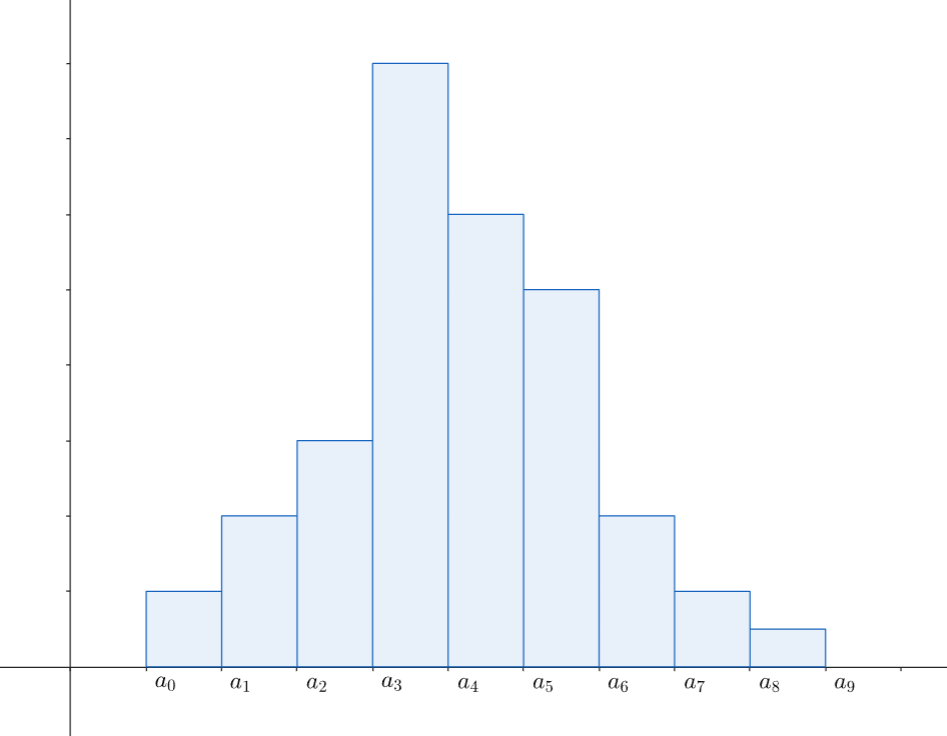
\includegraphics[width=0.7\textwidth]{mathstat/images/mathstat_2025_02_11_1}
    \end{center}

    Визуально можно сделать гипотезу, как ведет себя распределение. 

    \begin{MyTheorem}
        \Ths Гистограмма поточечно сходится к теоретической плотности
    \end{MyTheorem}

    \item Полигон

    На оси абсцисс отмечаем значения частотного вариационного ряда, по оси ординат - их частоты. 
    Получившиеся точки соединяем отрезками

    \begin{center}
        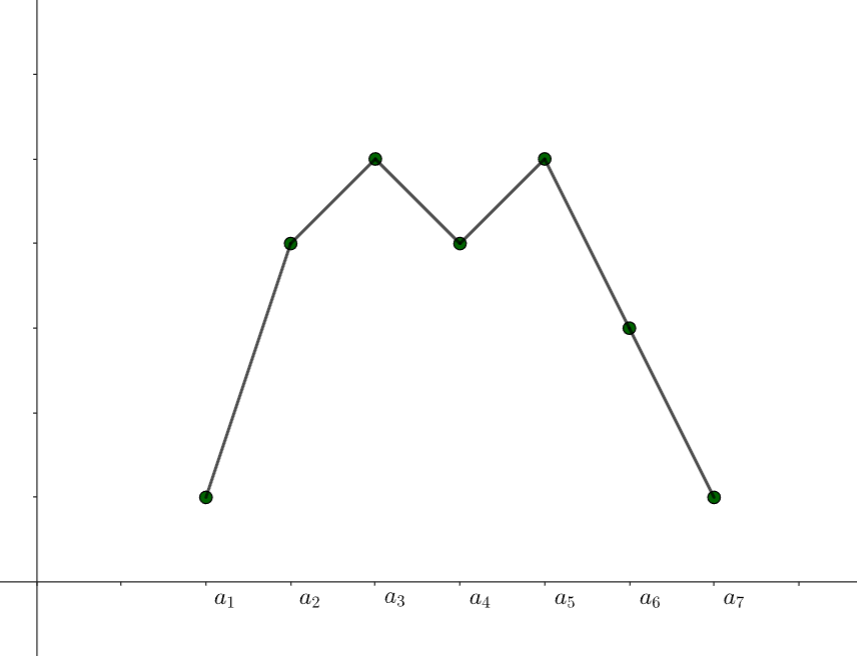
\includegraphics[width=0.7\textwidth]{mathstat/images/mathstat_2025_02_11_2}
    \end{center}

    \item Выборочная функция распределения

    На основе таблицы строится график функции распределения

    \begin{center}
        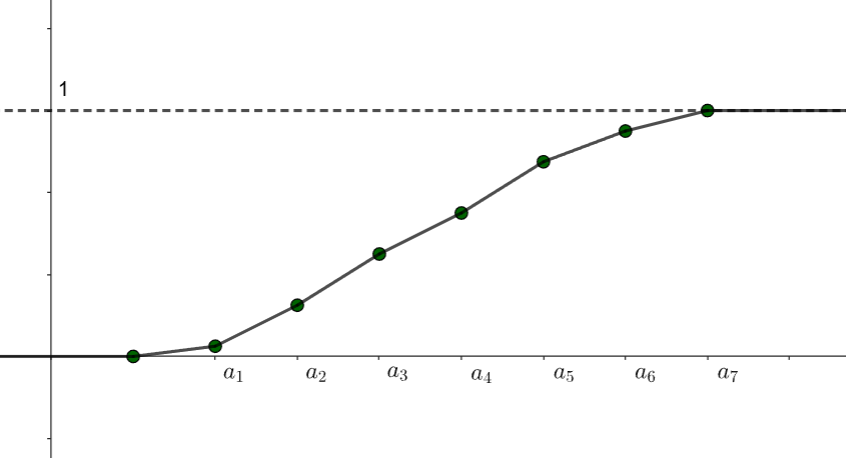
\includegraphics[width=0.7\textwidth]{mathstat/images/mathstat_2025_02_11_3}
    \end{center}

    Она может быть ступенчатой, ломаной или соединена по усмотрению

\end{itemize}





% end mathstat_2025_02_11.tex

% begin mathstat_2025_02_18.tex





\section{Лекция 2.}

\subsection{Точечная оценка}

Пусть имеется выборка $\vec{X} = (X_1, X_2, \dots, X_n)$ объемом $n$

Пусть требуется найти приближенную оценку $\theta^*$ неизвестного параметра $\theta$

Находим ее при помощи некоторой функции обработки данных $\theta^* = \theta^*(X_1, \dots, X_n)$

\Def Такая функция называется статистикой

\Defs А оценка $\theta^*$ называется точечной оценкой

\subsubsection{Свойство точечных оценок}

\begin{enumerate}
    \item Состоятельность

    \Defs Статистика $\theta^* = \theta^*(X_1, \dots, X_n)$ неизвестного параметра называется
    состоятельной, если $\theta^* \overset{p}{\longrightarrow} \theta$ при $n \to \infty$

    \mediumvspace

    \item Несмещенность

    \Defs Оценка $\theta^*$ параметра $\theta$ называется несмещенной, если 
    математическое ожидание $E \theta^* = \theta$
    
    \Notas Оценка $\theta^*$ называется асимптотически несмещенной, если 
    $E \theta^* \overset{p}{\longrightarrow} \theta$ при $n \to \infty$

    \mediumvspace

    \item Эффективность 

    \Defs Оценка $\theta^*_1$ не хуже $\theta^*_2$, если $E (\theta^*_1 - \theta)^2 \leq E (\theta^*_2 - \theta)^2$.
    Или, если $\theta^*_1$ и $\theta^*_2$ несмещенные, то $D \theta^*_1 \leq D \theta^*_2$

    \Defs Оценка $\theta^*$ называется эффективной, если она не хуже всех остальных оценок

    \Notas Не существует эффективной оценки в классе всех возможных оценок

    \begin{MyTheorem}
        \Ths В классе несмещенных оценок существует эффективная оценка
    \end{MyTheorem}

    \mediumvspace

    \item Асимптотическая нормальность

    \Defs Оценка $\theta^*$ параметра $\theta$ называется асимптотически нормальной, если 
    $\sqrt{n} (\theta^* - \theta) \rightrightarrows N(0, \sigma^2 (\theta))$ при $n \to \infty$
    
\end{enumerate}

\subsection{Точечные оценки моментов}

\Def Выборочным средним $\overline{x}$ называется величина $\overline{x} = \frac{1}{n} \sum_{i = 1}^n X_i$

\Defs Выборочной дисперсией $D^*$ называется величина $D^* = \frac{1}{n} \sum_{i = 1}^n (X_i - \overline{x})^2$

\Defs Исправленной дисперсией $S^2$ называется величина $S^2 = \frac{n}{n - 1} D^* = \frac{1}{n - 1} \sum_{i = 1}^n (X_i - \overline{x})^2$

\Defs Выборочным средним квадратическим отклонением называется величина $\sigma^* = \sqrt{D^*}$

\Defs Исправленным средним квадратическим отклонением называется величина $S = \sqrt{S^2}$

\Defs Выборочным $k$-ым моментом называется величина $\overline{x^k} = \frac{1}{n} \sum_{i = 1}^n X_i^k$

\Defs Модой $\mathrm{Mo}^*$ называется варианта $x_k$ с наибольшей частотой $n_k = \max_i (n_1, n_2, \dots, n_m)$

\Defs Выборочной медианой $\mathrm{Me}^*$ называется варианта $x_i$ в середине вариационного ряда $\begin{cases}\mathrm{Me}^* = 
X_{(k)}, & \text{если } n = 2k - 1 \\ \frac{X_{(k)} + X_{(k + 1)}}{2}, & \text{если } n = 2k\end{cases}$

\begin{MyTheorem}
    \Ths $\overline{x}$ - состоятельная несмещенная оценка теоретического матожидания $ЕX = a$

    1) $E \overline{x} = a$

    2) $\overline{x} \overset{p}{\longrightarrow} a$ при $n \to \infty$
\end{MyTheorem}

\begin{MyProof}
    1) $E \overline{x} = E\left(\frac{X_1 + \dots + X_n}{n}\right) = \frac{1}{n} \sum_{i = 1}^n E X_i = 
    \frac{1}{n} n E X_1 = E X_1 = a$

    2) $\overline{x} = \frac{\overline{x}_1 + \dots + \overline{x}_n}{n} \overset{p}{\longrightarrow} a$ 
    согласно Закону Больших Чисел
\end{MyProof}

\Nota Если второй момент конечен, то $\overline{x}$ - асимптотически нормальная оценка. По ЦПТ $\frac{S_n - n E X_1}{\sqrt{n} \sqrt{D X_1}} = \sqrt{n} \frac{\overline{x} - E X_1}{\sqrt{D X_1}} \rightrightarrows N(0, 1)$
или $\sqrt{n} (\overline{x} - E X_1) \rightrightarrows N(0; D X_1)$

\begin{MyTheorem}
    \Ths Выборочный $k$-ый момент является состоятельной несмещенной оценкой теоретического $k$-ого момента

    1) $\overline{E X^k} = E X^k$

    2) $\overline{X^k} \overset{p}{\longrightarrow} X^k$
\end{MyTheorem}

Это следует из предыдущей теоремы, если взять $X^k$ вместо $X$

\begin{MyTheorem}
    \Ths Выборочной дисперсией $D^*$ и $S^2$ являются состоятельными оценками теоретической дисперсией, при этом $D^*$ - смещенная оценка, а
    $S^2$ - несмещенная оценка
\end{MyTheorem}

\begin{MyProof}
    Заметим, что $D^* = \overline{X^2} - \overline{X}^2$

    $E D^* = E(\overline{X^2} - \overline{X}^2) = E\overline{X^2} - E (\overline{X}^2) = 
    E X^2 - E (\overline{X}^2)$

    Так как $D \overline{X} = E(\overline{X^2}) - (E \overline{X})^2$, то $E X^2 - E (\overline{X}^2) = 
    E X^2 - ((E\overline{X})^2 + D\overline{X}) = (E X^2 - EX) - D\overline{X} = D X - D \overline{X} = D X - D \left(\frac{X_1 + \dots + X_n}{n}\right) = 
    DX - \frac{1}{n^2} \sum_{i = 1}^n D X_i = DX - \frac{1}{n^2} n D X_1 = DX - \frac{1}{n} DX = \frac{n - 1}{n} DX$, то есть $D^*$ - смещенная вниз оценка

    $E S^2 = E(\frac{n}{n - 1} D^*) = \frac{n}{n - 1} \frac{n - 1}{n} DX = DX \Longrightarrow S^2$ - несмещенная вниз оценка 

    2. $D^* = \overline{X^2} - \overline{X}^2 \overset{p}{\longrightarrow} E X^2 - (E X)^2 = DX$ - состоятельная оценка

    $S^2 = \frac{n}{n - 1} D^* \overset{p}{\longrightarrow} DX$
\end{MyProof}

\Nota Отсюда видим, что выборочная дисперсия - асимптотически несмещенная оценка. Поэтому при большом (обычно не меньше 100) объеме выборке можно
считать обычную выборочную дисперсию

\subsection{Метод моментов (Пирсона)}

Постановка задачи: пусть имеется выборка объема $n$ неизвестного распределения, но известного типа,
которое задается $k$ параметрами: $\theta = (\theta_1, \theta_2, \dots, \theta_k)$. Требуется дать оценки данным
неизвестным параметрам

Идея метода состоит в том, что сначала находим оценки $k$ моментов, а затем с помощью теоретических формул
из теории вероятности даем оценки этих параметров

Пусть $\vec{X}$ - выборка из абсолютно непрерывного распределения $F_\theta$ с плотностью известного типа, 
которая задается $k$ параметрами $f_\theta (x, \theta_1, \dots, \theta_k)$

Тогда теоретические моменты находим по формуле $m_i = \int_{-\infty}^{\infty} x^i f_\theta (x, \theta_1, \dots, \theta_k) dx = h_i(\theta_1, \dots, \theta_n)$

Получаем систему из $k$ уравнений с $k$ неизвестными. В эти уравнения подставляем найденные оценки
моментов и, решая получившуюся систему уравнений, находим нужные оценки параметров

$\begin{cases}
    \overline{x} = h_1(\theta_1^*, \dots, \theta_n^*) \\ 
    \overline{x^2} = h_2(\theta_1^*, \dots, \theta_n^*) \\ 
    \dots \\
    \overline{x^k} = h_k(\theta_1^*, \dots, \theta_n^*) \\ 
\end{cases}$

\Nota Оценки по методу моментов как правило состоятельные, но часто смещенные

\Ex Пусть $X \in U(a, b)$. Обработав статданные, нашли оценки первого и второго моментов:

$\overline{x} = 2.25; \overline{x^2} = 6.75$

Найти оценки параметров $a^*, b^*$

Плотность равномерного распределения $f_{(a, b)} (x) = \begin{cases}0, & x < a \\ \frac{1}{b - a} & a \leq x \leq b, \\ 0, x > b\end{cases}$

$EX = \int_a^b x \frac{1}{b - a} dx = \frac{a + b}{2}$

$EX = \int_a^b x^2 \frac{1}{b - a} dx = \frac{a^2 + ab + b^2}{3}$

\mediumvspace

Получаем:

$\begin{cases}
    \overline{x} = \frac{a^* + b^*}{2} \\ 
    \overline{x^2} = \frac{a^*^2 + a^* b^* + b^*^2}{3} \\ 
\end{cases} \Longleftrightarrow \begin{cases}
    \frac{a^* + b^*}{2} = 4.5 \\ 
    a^*^2 + a^* b^* + b^*^2 = 20.25 \\ 
\end{cases} \Longleftrightarrow \begin{cases}
    \frac{a^* + b^*}{2} = 4.5 \\ 
    a^* b^* = 0 \\ 
\end{cases} \Longleftrightarrow \begin{cases}
    a^* = 0 \\ 
    b^* = 4.5 \\ 
\end{cases}$




% end mathstat_2025_02_18.tex

% begin mathstat_2025_02_25.tex





\section{Лекция 3.}

\subsection{Метод максимального правдоподобия}

Пусть имеется выборка $\vec{X} = (X_1, \dots, X_n)$ из распределения известного типа, определяемого неизвестными параметрами 
$\theta = (\theta_1, \dots, \theta_n)$

Идея метода состоит в следующем: подбираем параметры таким образом, чтобы вероятность получения
данной выборки при случайном эксперименте была наибольшей.

Если распределение дискретное, то $P_{\theta} (X_1 = x_1, X_2 = x_2, \dots, X_n = x_n) = P(X_1 = x_1) \dots P(X_n = x_n)$

\Def Функцией правдоподобия $L(\vec{X}, \theta)$ называется функция $L(\vec{X}, \theta) = P(X_1 = x_1) \dots P(X_n = x_n) = \prod_{i = 1}^n P(X_i = x_i)$ при дискретном распределении

и $L(\vec{X}, \theta) = f_\theta(x_1) \dots f_\theta(x_n) = \prod_{i = 1}^n f_\theta(x_i)$ в абсолютно непрерывном распределении

\Def Логарифмической функцией правдоподобия называется функция $\ln L(\vec{X}, \theta)$

\Nota Так как $y = \ln x$ возврастающая функция, точки максимума совпадают, а такую функцию правдоподобия становится легче дифференцировать

\Def Оценкой максимального правдоподобия $\hat{\theta}$ называется значение $\theta$, при котором функция правдоподобия 
$L(\vec{X}, \theta)$ достигает наибольшего значения (при фиксированных значениях выборки)

\ExN{1} Пусть $\vec{X} = (X_1, \dots, X_n)$ - выборка из распределения Пуассона $\Pi_\lambda$ с неизвестным $\lambda > 0$

\Mem Для распределения Пуассона $P(X = x_i) = \frac{\lambda^{x_i}}{x_i!} e^{-\lambda}$

Получаем функцию максимального правдоподобия $L(\vec{X}, \lambda) = \prod_{i = 1}^n \frac{\lambda^{x_i}}{x_i!} e^{-\lambda} = 
\frac{\lambda^{\sum_{i = 1}^n x_i}}{\prod_{i = 1}^n x_i!} e^{-n\lambda} = \frac{\lambda^{n \overline{x}}}{\prod_{i = 1}^n x_i!} e^{-n\lambda}$

$\ln L(\vec{X}, \lambda) = n \overline{x} \ln \lambda - \ln \prod_{i = 1}^n x_i! - n\lambda$

$\frac{\partial \ln L}{\partial \lambda} = \frac{n \overline{x}}{\lambda} - n = 0 \Longrightarrow \hat{\lambda} = \overline{x}$ - оценка максимального правдоподобия

Убедимся, что этот экстремум - максимум: $\frac{\partial^2 \ln L}{\partial \lambda^2} = -\frac{n \overline{x}}{\lambda} < 0 \Longrightarrow \hat{\lambda} = \overline{x}$ - точка максимума

\ExN{2} Пусть $(X_1, \dots, X_n)$ из $N(a, \sigma^2)$

$f_{a, \sigma^2} (x) = \frac{1}{\sigma \sqrt{2\pi}} e^{-\frac{(x - a)^2}{2\sigma^2}}$

$L(\vec{X}, a, \sigma^2) = \prod_{i = 1}^n \frac{1}{\sigma \sqrt{2\pi}} e^{-\frac{(x_i - a)^2}{2\sigma^2}} = 
\frac{1}{\sigma^n (2\pi)^{\frac{n}{2}}} e^{-\frac{\sum_{i = 1}^n (x_i - a)^2}{2\sigma^2}}$

$\ln L(\vec{X}, a, \sigma^2) = -n\ln \sigma - \frac{n}{2} \ln 2\pi - \frac{1}{2\sigma^2}\sum_{i = 1}^n (x_i - a)^2$

$\frac{\partial \ln L}{\partial a} = -\frac{1}{2\sigma^2} \sum_{i = 1}^n -2(x_i - a) = \frac{1}{\sigma^2} \sum_{i = 1}^n (x_i - a) = \frac{n\overline{x} - na}{\sigma^2}$

$\frac{\partial \ln L}{\partial \sigma} = -\frac{n}{\sigma} - \sum_{i = 1}^n (x_i - a)^2 \frac{1}{2} \cdot (-2) \cdot \sigma^{-3} = \frac{1}{\sigma^3} \sum_{i = 1}^n (x_i - a)^2 - \frac{n}{\sigma}$

$\begin{cases}
    \frac{n\overline{x} - na}{\sigma^2} = 0 \\
    \frac{1}{\sigma^3} \sum_{i = 1}^n (x_i - a)^2 - \frac{n}{\sigma} = 0
\end{cases} \Longrightarrow \begin{cases}
    \hat{a} = \overline{x} \\
    \widehat{\sigma^2} = \frac{1}{n} \sum_{i = 1}^n (x_i - a)^2 = D^*
\end{cases} $

\ExN{3} Пусть $(X_1, \dots, X_n)$ из $U(0, \theta)$. Найти оценку $\theta$ этого распределения.

Воспользуемся методом моментов:

$EX = \frac{a + b}{2} = \frac{\theta}{2} \Longrightarrow \overline{x} = \frac{\theta^*}{2} \Longrightarrow \theta^* = 2\overline{x}$

Воспользуемся методом максимального правдоподобия:

$f_\theta = \begin{cases}0, & x < 0 \\ \frac{1}{\theta}, & 0 \leq x \leq \theta \\ 0, & x > \theta \end{cases}$

$X_{(n)} = \max_i (X_1, \dots, X_n)$

$L(\vec{X}, \theta) = \prod_{i = 1}^n f_\theta (x_i) = 
\begin{cases}
    0, & \text{если } \theta < X_{(n)} \\ 
    \frac{1}{\theta^n}, & \text{если } \theta \geq X_{(n)}
\end{cases}$

$L(\vec{X}, \theta)$ достигает наибольшего значения при наименьшем значении $\theta^n$, то есть при $\hat{\theta} = X_{(n)}$

Сравним оценки:

$\theta^* = 2 \overline{x}$ - несмещенная оценка, так как $E\theta^* = 2E\overline{x} = 2E X = \theta$

$E(\theta^* - \theta)^2 = D\theta^* = D2\overline{x} = 4D\overline{x} = 4\frac{D\overline{x}}{n} = \frac{4}{n}\frac{\theta^2}{12} = \frac{\theta^2}{3n}$

Изучим распределение $X_{(n)}$: $F_{X_{(n)}}(x) = P(X_{(n)} < x) = P(X_1 < x, X_2 < x, \dots, X_n < x) = 
P(X_1 < x) \dots P(X_n < x) = F_{X_1}(x) \dots F_{X_n}(x) = F^n_{(x_1)}(x)$

$F_{X_1} (x) = \begin{cases}
    0, & x < 0 \\
    \frac{x}{\theta}, & 0 \leq x \leq \theta \\
    1, & x > \theta
\end{cases} \Longrightarrow F_{X_(n)}(x) = \begin{cases}
    0, & x < 0 \\
    \frac{x^n}{\theta^n}, & 0 \leq x \leq \theta \\
    1, & x > \theta
\end{cases} \Longrightarrow f_{X_(n)}(x) = \begin{cases}
    0, & x < 0 \\
    n\frac{x^{n - 1}}{\theta^n}, & 0 \leq x \leq \theta \\
    1, & x > \theta
\end{cases}$

$EX_{(n)} = \int_0^\theta x \cdot \frac{nx^{n - 1}}{\theta^n} dx = \frac{n}{\theta^n} \int_0^\theta x^n dx = \frac{n x^{x + 1}}{\theta^n (n + 1)} \Big|_0^\theta = 
\frac{n\theta}{n + 1}$ - смещенная вниз оценка

$\tilde{\theta} = \frac{n + 1}{n} X_{(n)}$ - несмещенная оценка (будем считать, что эффективность не изменилась)

$E\tilde{\theta}^2 = E(\frac{n + 1}{n} X_{(n)})^2 = \frac{(x + 1)^2}{n^2} E X_{(n)} = \frac{(n + 1)^2}{n^2} \int_0^\theta x^2 \frac{n x^{n - 1}}{\theta^n} dx = 
\frac{(n + 1)^2 \theta^2}{n (n + 2)}$

$D\tilde{\theta} = E\tilde{\theta}^2 - (E\tilde{\theta})^2 = \frac{\theta^2}{n(n + 2)}$

$D\tilde{\theta} = \frac{\theta^2}{n(n + 2)} < \frac{\theta^2}{3n} = D\theta^*$

Таким образом, оценка по методу правдоподобия сходится быстрее, чем оценка по методу моментов, поэтому она лучше

Отсюда следует, что при равномерном распределении выборочное среднее не является эффективной оценкой
для математического ожидания; вместо нее половина максимального элемента выборки будет лучше

\Nota Эффективной здесь будет несмещенная оценка $\frac{n + 1}{2n} X_{(n)}$

В общем случае для $U(a, b)$ будет такая эффективная оценка матожидания - $\frac{X_{(1)} + X_{(n)}}{2}$, длины интервала - $\frac{n + 1}{n - 1} (X_{(n)} - X_{(1)})$

\Nota При методе максимального правдоподобия обычно получаем состоятельные и эффективные оценки, но часто смещенные

\subsection{Неравенство Рао-Крамера}

Пусть $X \in F_\theta$ - семейство распределений с параметром $\theta \in \Real$

\Def Носителем семейства распределений $F_\theta$ называется множество $C \subset \Real$
такое, что $P(X \in C) = 1 \ \forall X \in F_\theta$

$f_\theta(x) = \begin{cases}
    \text{плотность } f_\theta(x) \text{ при непрерывном распределении} \\
    P_\theta(X = x) \text{ при дискретном распределении}
\end{cases}$

\Def Информацией Фишера $I(\theta)$ семейства распределений $F_\theta$ называется величина 
$I(\theta) = E\left(\frac{\partial}{\partial \theta} \ln f_\theta(X)\right)^2$ при условии, что
она существует

\Def Семейство распределений $F_\theta$ называется регулярным, если:

\begin{itemize}
    \item существует носитель $C$ семейства $F_\theta$ такой, что $\forall x \in C \ $ функция $\ln f_\theta(x)$ непрерывно дифференцируема по $\theta$
    \item информация Фишера $I(\theta)$ существует и непрерывна по $\theta$
\end{itemize}

\begin{MyTheorem}
    \Ths Пусть $(X_1, \dots, X_n)$ - выборка объема $n$ из регулярного семейства $F_\theta$,

    $\theta^* = \theta^*(X_1, \dots, X_n)$ - несмещенная оценка параметра $\theta$, дисперсия которой
    $D\theta^*$ ограничена в любой замкнутой ограниченной области параметра $\theta$

    Тогда \fbox{$D\theta^* \geq \frac{1}{n I(\theta)}$}
\end{MyTheorem}

\underline{Следствие}: если при данных услових получили $D\theta^* = \frac{1}{n I(\theta)}$, то оценка $\theta^*$ является эффективной 
(то есть дальше улучшать уже некуда)

\Ex Пусть $(X_1, \dots, X_n)$ из $N(a, \sigma^2)$ (то есть $F_a = N(a, \sigma^2)$, $\sigma^2$ зафиксируем)

Проверим эффективность $a^* = \overline{x}$

Плотность $f_a(x) = \frac{1}{\sigma \sqrt{2\pi}} e^{-\frac{(x - a)^2}{2\sigma^2}}$, носитель - вся прямая $\Real$

$\ln f_a(x) = -\ln \sigma - \frac{1}{2} \ln 2\pi - \frac{(x - a)^2}{2\sigma^2}, \quad\quad a \in (-\infty, \infty)$

$\frac{\partial}{\partial a} \ln f_a(x) = \frac{1}{2\sigma^2} \cdot 2(x - a) = \frac{x - a}{\sigma^2}$ - непрерывна для всех $a \in \Real$

$I(a) = E\left(\frac{\partial}{\partial a} \ln f_a(X)\right)^2 = E\left(\frac{X - a}{\sigma^2}\right)^2 = \frac{1}{\sigma^4} E(X - a)^2 = \frac{E(X - EX)^2}{\sigma^4} = 
\frac{DX}{\sigma^4} = \frac{1}{\sigma^2}$ - непрерывна по $a$

Из этого следует, что $N(a, \sigma^2)$ - регулярное семейство относительно параметра $a$

$Da^* = D\overline{x} = \frac{DX}{n} = \frac{\sigma^2}{n}$ - ограничена по параметру $a$

По неравенству Рао-Крамера $Da^* = \frac{\sigma^2}{n} =\joinrel= \frac{1}{nI(a)} = \frac{1}{n} \sigma^2$; из 
этого следует, что $a^*$ - эффективная оценка параметра $a$

\Nota Аналогично можно показать, что $S^2$ - несмещенная эффективная оценка для параметра $\sigma^2$



% end mathstat_2025_02_25.tex

% begin mathstat_2025_03_04.tex





\section{Лекция 4.}

\subsection{Основные распределения математической статистики}

\Def Случайная величина имеет нормальное распределение $\xi \in N(a, \sigma^2)$ с параметрами $a$ и $\sigma^2$, если
ее плотность имеет вид $f_\xi(x) = \frac{1}{\sigma\sqrt{2\pi}} e^{-\frac{(x - a)^2}{2\sigma^2}}$

На практике нормальное распределение встречается чаще всего в силу ЦПТ

\Def Распределение $N(0, 1)$ с параметрами $a = 0, \sigma^2 = 1$ называется стандартным нормальным распределением. 
Его плотность равна $\varphi(x) = \frac{1}{\sqrt{2\pi}} e^{-\frac{x^2}{2}}$. 
В дальнейшем такую случайную величину будем называть стандартной нормалью

\underline{Свойства}

\begin{enumerate}
    \item $a = E\xi \qquad \sigma^2 = D\xi$

    \item Линейность: $\xi \in N(a, \sigma^2)$, то $\eta = b \xi + \gamma \in N(ab + \gamma, b^2 \sigma^2)$

    \item Стандартизация: Если $\xi \in N(a, \sigma^2)$, то $\eta = \frac{\xi - a}{\sigma} \in N(0, 1)$

    \item Устойчивость относительно суммирования: если $\xi_1 \in N(a_1, \sigma^2_1)$, $\xi_2 \in N(a_2, \sigma^2_2)$, независимы
    то $\xi_1 + \xi_2 \in N(a_1 + a_2, \sigma^2_1 + \sigma^2_2)$
\end{enumerate}

\subsubsection{Распределение \enquote{хи-квадрат}}

\Def Распределение \enquote{хи-квадрат} $H_n$ со степенями свободы $n$ называется распределение
суммы квадратов независимых стандартных нормальных величин: $\chi^2_n = X_1^2 + X_2^2 + \dots + X_n^2$, 
где $X \in N(0, 1)$ и независимы

\underline{Свойства}

\begin{enumerate}
    \item $E\chi^2_n = n$

    \begin{MyProof}
        Так как $\forall i \ X_i \in N(0, 1)$, то $E X_i^2 = D X_i^2 + (EX_i)^2 = 1 \Longrightarrow E(X_i^2 + \dots X_n^2) = \sum_{i = 1}^n X_i^2 = n$
    \end{MyProof}

    \item Устойчивость относительно суммирования: если $X \in H_n$, $Y \in H_m$, независимы, то $X + Y \in H_{n + m}$ (по определению) 


    \item $\frac{\chi_k^2}{k} \overset{p}{\underset{k \to \infty}{\longrightarrow}} 1$ (по Закону Больших Чисел)
\end{enumerate}

\subsubsection{Распределение Стьюдента}

\Def Пусть $X_0, X_1, \dots, X_k$ - независимые стандартные нормальные величины. 
Распределением Стьюдента $T_k$ с $k$ степенями свободы называется распределение случайной величины 
$t_k = \frac{X_0}{\sqrt{\frac{1}{k} (X_1^2 + \dots + X_k^2)}} = \frac{X_0}{\sqrt{\frac{\chi_k^2}{k}}}$

\underline{Свойства}

\begin{enumerate}
    \item $Et_k = 0$ - в силу симметрии

    \item $t_k \rightrightarrows N(0, 1)$ (на практике при $k \geq 100$ распределение Стьюдента можно считать стандартным нормальным)
\end{enumerate}

\subsubsection{Распределение Фишера-Снедекера}

\Def Распределением Фишера-Снедекера $F_{n,m}$ (другое название - F-распределение) со степенями свободы $n$ и $m$ называется распределение случайной величины 
$f_{n,m} = \frac{\frac{\chi^2_n}{n}}{\frac{\chi^2_m}{m}}$, где $\chi_n^2$ и $\chi_m^2$ - независимые случайные величины с распределением \enquote{хи-квадрат}

\underline{Свойства}

\begin{enumerate}
    \item $E f_{n,m} = \frac{n}{n - 2}$

    \item $f_{n,m} \overset{p}{\underset{n, m \to \infty}{\longrightarrow}} 1$
\end{enumerate}


\subsection{Математическое ожидание и дисперсия случайного вектора}

Пусть $\vec X = \begin{pmatrix}X_1 \\ \vdots \\ X_n\end{pmatrix}$ - случайный вектор, 
где случайная величина $X_i$ - компонента (координата) случайного вектора

\Def Математическим ожидание случайного вектора называется вектор с координатами из математических ожиданий компонент: 
$E \vec X = \begin{pmatrix}E X_1 \\ \vdots \\ E X_n\end{pmatrix}$

\Def Дисперсией случайного вектора (или матрицей ковариаций) случайного вектора $\vec X$ называется
матрица $D \vec X = E (\vec X - E \vec X) (\vec X - E \vec X)^T$, состоящая из элементов $d_{ij} = \mathrm{cov} (X_i, X_j)$

\Notas На главной диагонали стоят дисперсии компонент: $d_{ii} = D X_i$

\Notas $D \vec X$ - симметричная положительно определенная матрица

\underline{Свойства}

\begin{enumerate}
    \item $E (A \vec X) = A E \vec X$

    \item $E (\vec X + \vec B) = E \vec X + \vec B$, где $\vec B$ - вектор чисел

    \item $D (A \vec X) = A \cdot D \vec X \cdot A^T$

    \item $D (\vec X + \vec B) = D \vec X$
\end{enumerate}

\subsection{Многомерное нормальное распределение}

\Def Пусть случайный вектор $\vec \xi = \begin{pmatrix}\xi_1 \\ \vdots \\ \xi_n\end{pmatrix}$ имеет вектор средних 
$\vec a = E \vec \xi$, $K$ - симметричная положительно определенная матрица. Вектор $\vec \xi$ 
имеет нормальное распределение в $\Real^n$ с параметрами $\vec a$ и $K$, если его плотность 
$f_{\vec \xi} (\vec X) = \frac{1}{\left(\sqrt{2\pi}\right)^n \sqrt{\det K}} e^{-\frac{1}{2} (\vec X - \vec a)^T K^{-1} (\vec X - \vec a)}$


\underline{Свойства}

\begin{enumerate}
    \item Матрица $K = D \vec \xi = \left(\mathrm{cov} (\xi_i, \xi_j)\right)$ - матрица ковариаций

    \item При $\vec a = \vec 0$ и $K = E$ имеем вектор из независимых стандартных нормальных величин

    \begin{MyProof}
        При $\vec a = \vec 0$ и $K = E$: $f_{\vec \xi} (X_1, \dots, X_n) = \frac{1}{\left(\sqrt{2\pi}\right)^n} 
        e^{-\frac{1}{2} \begin{pmatrix}X_1 & \dots & X_n\end{pmatrix} E \begin{pmatrix}X_1 & \dots & X_n\end{pmatrix}^T} = 
        \frac{1}{\left(\sqrt{2\pi}\right)^n} e^{-\frac{1}{2} (X_1^2 + \dots + X_n^2)} = 
        \frac{1}{\sqrt{2\pi}} e^{-\frac{1}{2} X_1^2} + \dots + \frac{1}{\sqrt{2\pi}} e^{-\frac{1}{2} X_n^2}$

        Так как плотность распалась на произведение плотностей стандартного нормального распределение, то все компоненты имеют стандартное нормальное распределение
    \end{MyProof}
\end{enumerate}

Далее вектором из независимых стандартных нормальных величин для краткости будем называть стандартным нормальным вектором

\begin{enumerate}
    \setcounter{enumi}{2}

    \item $\letsymbol \vec X$ - стандартный нормальный вектор, $B$ - невырожденная матрица, 
    тогда вектор $\vec Y = B \vec X + \vec a$ имеет многомерное нормальное распределение с параметрами $\vec a$ и $K = B B^T$

    \item $\letsymbol \vec Y \in N(\vec a, K)$. Тогда вектор $\vec X = B^{-1} (\vec Y - \vec a)$ - стандартный нормальный вектор, где $B = \sqrt{K}$

    \underline{Следствие}. Эквивалентное определение: Многомерное нормальное распределение - это то, которое получается из
    стандартного нормального вектора при помощи невырожденного преобразования и сдвиг

    \item $\letsymbol \vec X$ - стандартный нормальный вектор, $C$ - ортогональная матрица. Тогда $\vec Y = C \vec X$ - стандартный нормальный вектор

    \begin{MyProof}
        Так как $C$ - ортогональная, то $C^T = C^{-1}$. Тогда по третьему свойству $K = C C^T = E$, а по второму свойству $\vec Y$ - стандартный нормальный вектор
    \end{MyProof}

    \item $\letsymbol$ случайный вектор $\xi \in N(\vec a, K)$.
    Тогда его координаты независимы тогда и только тогда, когда они не коррелированы (то есть матрица ковариаций $K$ диагональная)

    % какого распределения величины
    \underline{Следствие}. Если плотность совместного распределения случайных величин $\xi$ и $\eta$ ненулевая, то они независимы тогда и только тогда, 
    когда их коэффициент корреляции равен нулю
\end{enumerate}

\subsection{Многомерная центральная предельная теорема}

\begin{MyTheorem} 
    \Ths Среднее арифметическое независимых одинаково распределенных случайных векторов слабо сходится к многомерному нормальному распределению
\end{MyTheorem}

\subsection{Лемма Фишера}

\begin{MyTheorem}
    Пусть вектор $\vec X$ - стандартный нормальный вектор, $C$ - ортогональная матрица, $\vec Y = C \vec X$.
    Тогда $\forall 1 \leq k \leq n - 1 \ $ случайная величина $T(\vec X) = \sum_{i = 1}^n X_i^2 - Y_1^2 - Y_2^2 - \dots Y_k^2$ 
    не зависит от $Y_1, Y_2, \dots, Y_k$ и имеет распределение \enquote{хи-квадрат} со степенями свободы $n - k$
\end{MyTheorem}

\begin{MyProof}
    Так как $C$ - ортогональное преобразование, то $\|\vec X\| = \|\vec Y\|$, то есть $\sum_{i = 1}^n X^2_i = \sum_{i = 1}^n Y^2_i \Longrightarrow
    T(\vec X) = \sum_{i = 1}^n X_i^2 - Y_1^2 - Y_2^2 - \dots Y_k^2 = Y^2_{k + 1} + \dots + Y^2_{n}$

    Согласно свойству 5 $Y_i \in N(0, 1)$ и независимы, то по определению \enquote{хи-квадрат} $T(\vec X) \in H_{n - k}$ и не зависит от $Y_1, \dots, Y_k$
\end{MyProof}

\subsection{Основная теорема}

Эта теорема также известна как \href{https://tvims.nsu.ru/chernova/ms/lec/node37.html}{основное следствие леммы Фишера}

\begin{MyTheorem}
    \Ths Пусть $(X_1, \dots, X_n)$ - выборка из нормального распределения $N(a, \sigma^2)$, $\overline{x}$ - выборочное среднее, $S^2$ - исправленная дисперсия.

    Тогда справедливы следующие высказывания:

    \begin{enumerate}
        \item $\sqrt{n} \frac{\overline{x} - a}{\sigma} \in N(0, 1)$
        
        \item $\sum_{i = 1}^n \frac{(X_i - a)^2}{\sigma^2} \in H_n$
        
        \item $\sum_{i = 1}^n \frac{(X_i - \overline{x})^2}{\sigma^2} = \frac{n D^*}{\sigma^2} = \frac{(n - 1) S^2}{\sigma^2} \in H_{n - 1}$

        \item $\sqrt{n} \frac{\overline{x} - a}{S} \in T_{n - 1}$
        
        \item $\overline{x}$ и $S^2$ независимы
    \end{enumerate}
\end{MyTheorem}

\begin{MyProof}
    \begin{enumerate}
        \item Так как $X_i \in N(a, \sigma^2)$, то $\sum_{i = 1}^n X_i \in N(na, n\sigma^2) \Longrightarrow \overline{x} \in N\left(a, \frac{\sigma^2}{n}\right) \Longrightarrow
        \overline{x} - a \in N\left(0, \frac{\sigma^2}{n}\right) \Longrightarrow \frac{\sqrt{n}}{\sigma} (\overline{x} - a) \in N(0, 1)$

        \item Так как $X_i \in N(a, \sigma^2)$, то $\frac{X_i - a}{\sigma} \in N(0, 1)$ и $\sum_{i = 1}^n \frac{(X_i - a)^2}{\sigma^2} \in H_n$ по определению
        
        \item $\sum_{i = 1}^n \frac{(X_i - \overline{x})^2}{\sigma^2} = \sum_{i = 1}^n \left(\frac{X_i - a}{\sigma} - \frac{\overline{x} - a}{\sigma}\right)^2 = 
        \sum_{i = 1}^n (z_i - \overline{z})^2$, где $z_i = \frac{X_i - a}{\sigma} \in N(0, 1)$, $\overline{z} = \frac{1}{n} \sum_{i = 1}^n z_i = \frac{\sum_{i = 1}^n X_i - na}{\sigma} = \frac{\overline{x} - a}{\sigma}$

        Поэтому можно считать, что изначально $X_i \in N(0, 1)$

        $T(\vec X) = \sum_{i = 1}^n \left(X_i - \overline{x}\right)^2 = n D^* = n (\overline{x^2} - \overline{x}^2) = \sum_{i = 1}^n X_i^2 - n\overline{x}^2 = \sum_{i = 1}^n X_i^2 - Y_1^2$, где $Y_1 = \sqrt{n} \overline{x} = \frac{X_1}{\sqrt{n}} + \dots + \frac{X_n}{\sqrt{n}}$

        Строчка $\left(\frac{1}{\sqrt{n}}, \dots, \frac{1}{\sqrt{n}}\right)$ имеет длину 1, поэтому ее можно дополнить до ортогональной матрицы $C$, тогда $Y_1$ - первая компонента $\vec Y = C \vec X$, 
        и согласно лемме Фишера $T(\vec X) = \sum_{i = 1}^n (X_i - \overline{X})^2 \in H_{n - 1}$

        
        \setcounter{enumi}{4}
        \item Согласно лемме Фишера $T(\vec X) = (n - 1) S^2$ не зависит от $Y_1 = \sqrt{n} \overline{x} \Longrightarrow S^2 $ и $\overline{x}$ - независимы
          
        \setcounter{enumi}{3}
        \item $\sqrt{n} \frac{\overline{x} - a}{S} = \sqrt{n} \frac{\overline{x} - a}{\sigma} \cdot \frac{1}{\sqrt{\frac{S^2 (n - 1)}{\sigma^2}} \cdot \frac{1}{n - 1}} = \frac{\sqrt{n} \frac{\overline{x} - a}{\sigma}}{\frac{\chi^2_{n - 1}}{n - 1}}$

        Так как по пятому пункту числитель и знаменатель независимы, по определению получаем распределение Стьюдента
    \end{enumerate}
\end{MyProof}






% end mathstat_2025_03_04.tex

% begin mathstat_2025_03_11.tex





\section{Лекция 5.}

\subsection{Квантильное распределение}

Предполагаем, что распределение абсолютно непрерывное и $F(x)$ - функция распределения

\DefN{1} Число $t_\gamma$ называется квантилем распределения уровня $\gamma$, если значения
функции распределения $F(t_\gamma) = \gamma$ или $P(X < t_\gamma) = \gamma$ ($t_\gamma = F^{-1}(\gamma)$)

% https://www.geogebra.org/calculator/ezemup66

\begin{center}
    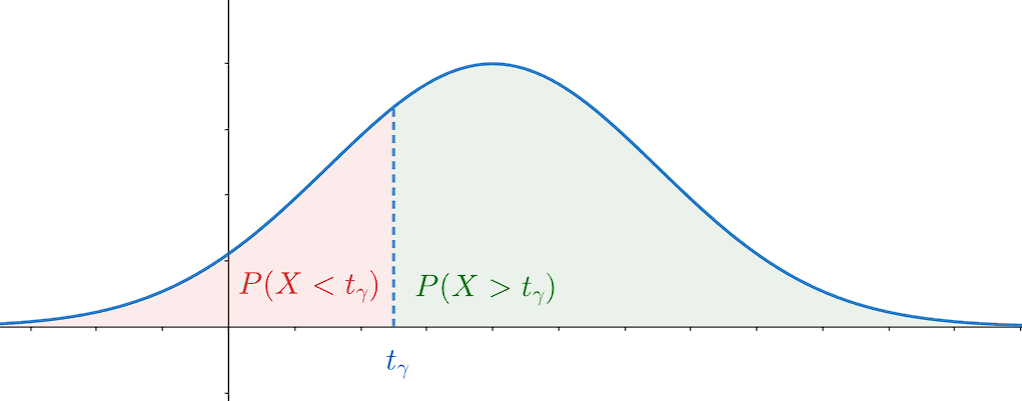
\includegraphics[width=15cm]{mathstat/images/mathstat_2025_03_11_1}
\end{center}

\Ex Медиана - квантиль уровня $\frac{1}{2}$

\DefN{2} Число $t_\alpha$ называется квантилем уровня значимости $\alpha$, если
$P(X > t_\alpha) = \alpha$ или $F(t_\alpha) = 1 - \alpha$

Ясно, что $\gamma = 1 - \alpha$

\subsection{Интервальные оценки}

Недостатки точечных оценок - неизвестно насколько они далеки от реального значения параметра и 
насколько им можно доверять. Особенно это заметно при малых выборках. Поэтому мы указываем интервал, в котором 
лежит этот параметр с заданной вероятностью (надежностью) $\gamma$. Такие оценки называются интервальными 
(доверительными)

\Def Интервал $(\theta^-_\gamma; \theta^+_\gamma)$ называется доверительным интервалом параметра $\theta$
надежности $\gamma$, если вероятность $P(\theta^-_\gamma < \theta < \theta^+_\gamma) = \gamma$

\Nota Если имеем дискретную случайную величину, то $P(\theta^-_\gamma < \theta < \theta^+_\gamma) \geq \gamma$

\Notas Так как параметр $\theta$ - константа, то бесмысленно говорить о его попадании в интервал. Правильно: 
доверительный интервал накрывает параметр $\theta$ с вероятностью $\gamma$

\NotaN{1} $\alpha = 1 - \gamma$ называется уровнем значимости доверительного интервала

\NotaN{2} Обычно пытаются строить симметричный доверительный интервал относительно несмещенной оценки $\theta^*$

\NotaN{3} Возникает вопрос, какой уровень $\gamma$ выбрать для исследования.
Стандартные уровени надежности $\gamma$: $0.9, \ 0.95, \ 0.99, \ 0.999$. Самый мейнстримный - $0.95$. 
В малых выборках используют $0.9$

Вспомним основную теорему:

\begin{MyTheorem}
    $\letsymbol (X_1, \dots, X_n)$ - выборка объема $n$ из $N(\alpha, \sigma^2)$

    $\overline{x}$ - выборочное среднее, $S^2$ - исправленная дисперсия, $D^*$ - выборочная дисперсия

    Тогда:

    \begin{enumerate}
        \item $\sqrt{n} \frac{\overline{x} - a}{\sigma} \in N(0, 1)$
        \item $\sum_{i = 1}^n \left(\frac{X_i - a}{\sigma}\right)^2 = \frac{n \tilde{\sigma^2}}{\sigma^2} \in H_n$, 
        где $n \tilde{\sigma^2} = \sum_{i = 1}^n (X_i - a)^2$
        \item $\sum_{i = 1}^n \left(\frac{X_i - \overline{x}}{\sigma}\right)^2 = \frac{(n - 1)S^2}{\sigma^2} = 
        \frac{nD^*}{\sigma^2} \in H_{n - 1}$
        \item $\sqrt{n} \frac{\overline{x} - a}{S} \in T_{n - 1}$
        \item $\overline{x}$ и $S^2$ - независимы
    \end{enumerate}
\end{MyTheorem}


\Nota Если $F(x)$ - функция симметричного относительно $x = 0$ распределения, то $P(|X| < t) = 2F(t) - 1$

% https://www.geogebra.org/calculator/msnwgfyp

\begin{center}
    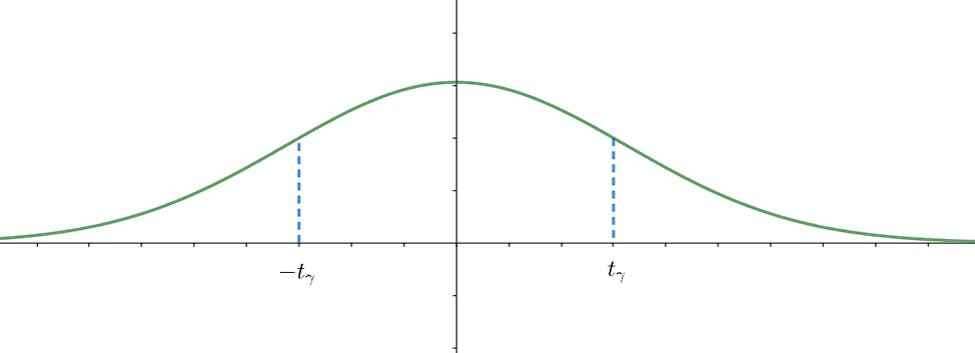
\includegraphics[width=15cm]{mathstat/images/mathstat_2025_03_11_2}
\end{center}

\subsection{Доверительные интервалы для параметров нормального распределения}

Пусть $\vec X = (X_1, \dots, X_n)$ - выборка объема $n$ из $N(a, \sigma^2)$. 
Хотим найти интервалы для параметров $a$ и $\sigma^2$

\begin{enumerate}[label*=\Roman*.]
    \item Доверительный интервал для параметра $a$ при известном значении $\sigma^2$

    По пункту 1 из теоремы $\sqrt{n} \frac{\overline{x} - a}{\sigma} \in N(0, 1)$ 

    $P\left(-t_\gamma < \sqrt{n} \frac{\overline{x} - a}{\sigma} < t_\gamma\right) = 
    P\left(\left|\sqrt{n} \frac{\overline{x} - a}{\sigma}\right| < t_\gamma\right) = 2F_0 (t_\gamma) - 1 = \gamma$

    $F_0(t_\gamma) = \frac{1 + \gamma}{2} \Longrightarrow t_\gamma$ - квантиль уровня 
    $\frac{1 + \gamma}{2}$ для $N(0, 1)$, где
    $F_0(x) = \frac{1}{\sqrt{2\pi}} \int_{-\infty}^{\infty} e^{-\frac{z^2}{2}} dz$

    Решая неравенство, получаем $-t_\gamma < \sqrt{n} \frac{\overline{x} - a}{\sigma} < t_\gamma$

    $-t_\gamma \frac{\sigma}{\sqrt{n}} < \overline{x} - a < t_\gamma \frac{\sigma}{\sqrt{n}}$

    $\overline{x} - t_\gamma \frac{\sigma}{\sqrt{n}} < a < \overline{x} + t_\gamma \frac{\sigma}{\sqrt{n}}$ - 
    симметричный интервал относительно $\overline{x}$

    Доверительный интервал надежности $\gamma$: $\left(\overline{x} - t_\gamma \frac{\sigma}{\sqrt{n}}, 
    \overline{x} + t_\gamma \frac{\sigma}{\sqrt{n}}\right)$, 
    где $t_\gamma$ - квантиль $N(0, 1)$ уровня $\frac{1 + \gamma}{2}$

    \item Доверительный интервал для параметра $a$ при неизвестном $\sigma^2$

    Из пункта 4 из теоремы $\sqrt{n} \frac{\overline{x} - a}{S} \in T_{n - 1}$

    $P\left(-t_\gamma < \sqrt{n} \frac{\overline{x} - a}{S} < t_\gamma\right) = P\left(\left|\sqrt{n} \frac{\overline{x} - a}{S}\right| < t_\gamma\right) = 2F_{T_{n - 1}}(t_\gamma) = \gamma$

    $F_{T_{n - 1}}(t_\gamma) = \frac{1 + \gamma}{2} \Longrightarrow t_\gamma$ - квантиль $T_{n - 1}$ уровня 
    $\frac{1 + \gamma}{2}$

    Аналогично с примером выше получаем интервал $\left(\overline{x} - t_\gamma \frac{S}{\sqrt{n}}, 
    \overline{x} + t_\gamma \frac{S}{\sqrt{n}}\right)$, 
    где $t_\gamma$ - квантиль $T_{n - 1}$ уровня $\frac{1 + \gamma}{2}$

    \item Доверительный интервал для параметра $\sigma^2$ при неизвестном $a$

    По пункту 3 из теоремы $\sum_{i = 1}^n \left(\frac{X_i - \overline{x}}{\sigma}\right)^2 = \frac{(n - 1)S^2}{\sigma^2} = 
    \frac{nD^*}{\sigma^2} \in H_{n - 1}$

    Пусть $\chi_1^2$ и $\chi_2^2$ - квантили $H_{n - 1}$ уровней $\frac{1 - \gamma}{2}$ и $\frac{1 + \gamma}{2}$

    Тогда $P\left(\chi_1^2 < \frac{(n - 1)S^2}{\sigma^2} < \chi_2^2\right) = F_{H_{n - 1}}(\chi_1^2) - F_{H_{n - 1}}(\chi_2^2) = \frac{1 - \gamma}{2} - \frac{1 + \gamma}{2} = \gamma$

    $\chi_1^2 < \frac{(n - 1)S^2}{\sigma^2} < \chi_2^2$

    $\frac{1}{\chi_2^2} < \frac{\sigma^2}{(n - 1)S^2} < \frac{1}{\chi_1^2}$

    $\frac{(n - 1)S^2}{\chi_2^2} < \sigma^2 < \frac{(n - 1)S^2}{\chi_1^2}$ или 
    $\frac{nD^*}{\chi_2^2} < \sigma^2 < \frac{nD^*}{\chi_1^2}$

    Получаем интервал $\left(\frac{(n - 1)S^2}{\chi_2^2}, \frac{(n - 1)S^2}{\chi_1^2}\right)$, где $\chi_1^2$ и $\chi_2^2$ - квантили $H_{n - 1}$ уровней $\frac{1 - \gamma}{2}$ и $\frac{1 + \gamma}{2}$

    \Nota Данный интервал не симметричен относительно неизвестного параметра $\sigma^2$

    \item Доверительный интервал для параметра $\sigma^2$ при известном $a$

    По пункту 2 из теоремы $\sum_{i = 1}^n \left(\frac{X_i - a}{\sigma}\right)^2 = \frac{n \tilde{\sigma^2}}{\sigma^2} \in H_{n - 1}$
    
    Пусть $\chi_1^2$ и $\chi_2^2$ - квантили $H_{n}$ уровней $\frac{1 - \gamma}{2}$ и $\frac{1 + \gamma}{2}$

    Тогда $P\left(\chi_1^2 < \frac{n \tilde{\sigma^2}}{\sigma^2} < \chi_2^2\right) = F_{H_{n}}(\chi_1^2) - F_{H_{n}}(\chi_2^2) = \frac{1 - \gamma}{2} - \frac{1 + \gamma}{2} = \gamma$

    Аналогично получаем интервал $\left(\frac{n \tilde{\sigma^2}}{\chi_2^2}, \frac{n \tilde{\sigma^2}}{\chi_1^2}\right)$, 
    где $\chi_1^2$ и $\chi_2^2$ - квантили $H_{n}$ уровней $\frac{1 - \gamma}{2}$ и $\frac{1 + \gamma}{2}$, $n \tilde{\sigma^2} = \sum_{i = 1}^n (X_i - a)^2$

    \Nota $\tilde{\sigma^2} - D^* = \frac{1}{n} \sum_{i = 1}^n (X_i - a)^2 - \frac{1}{n} \sum_{i = 1}^n (X_i - \overline{x})^2 = 
    \frac{1}{n} \sum_{i = 1}^n (X_i^2 - 2aX_i + a^2 - X_i^2 + 2 \overline{x} X_i - \overline{x}^2) = 
    \frac{1}{n} (na^2 - 2a n \overline{x} + 2 \overline{x} \cdot n \overline{x} - n \overline{x}^2) = 
    a^2 - 2a \overline{x} + \overline{x}^2 = (a - \overline{x})^2 \Longrightarrow \tilde{\sigma^2} = D^* + (a - \overline{x})^2$

    Получаем $\left(\frac{n (D^* + (a - \overline{x})^2)}{\chi_2^2}, \frac{n (D^* + (a - \overline{x})^2)}{\chi_1^2}\right)$

\end{enumerate}

\subsection{Асимптотические доверительные интервалы}

\Def Интервал $(\theta^-_\gamma, \theta^+_\gamma)$ называется асимптотическим доверительным интервалом параметра $\theta$ 
уровня $\gamma$, если $P(\theta^-_\gamma < \theta < \theta^+_\gamma) \underset{n \to \infty}{\longrightarrow} \gamma$

\Ex Доверительный интервал вероятности события $A$

Пусть $p = P(A), q = 1 - p, n$ - число испытаний или объем выборки $(X_1, \dots, X_n)$, где $X_i \in \{0, 1\}$

$p^* = \frac{n_A}{n} = \overline{x}$ - оценка $p$

Согласно Центральной предельной теореме $\sqrt{n} \frac{p^* - p}{D X_1} = \sqrt{n} \frac{p^* - p}{\sqrt{pq}} \rightrightarrows N(0, 1)$

Так как $p^* \overset{p}{\longrightarrow} p$, то $\sqrt{n} \frac{p^* - p}{\sqrt{p^* (1 - p^*)}} = 
\sqrt{n} \underset{\rightrightarrows N(0, 1)}{\underbrace{\frac{p^* - p}{\sqrt{p (1 - p)}}}} \underset{\overset{p}{\longrightarrow} 1}{\underbrace{\frac{\sqrt{p (1 - p)}}{\sqrt{p^* (1 - p^*)}}}} \rightrightarrows N(0, 1)$


$P\left(\left|\sqrt{n} \frac{p^* - p}{\sqrt{p^* (1 - p^*)}}\right| < t_\gamma\right) \underset{n \to \infty}{\longrightarrow} 2F_0(t_\gamma) - 1 = \gamma$

$F_0(t_\gamma) = \frac{1 + \gamma}{2}$, $t_\gamma$ - квантиль $N(0, 1)$ уровня $\frac{1 + \gamma}{2}$

Получаем $\left|\sqrt{n} \frac{p^* - p}{\sqrt{p^* (1 - p^*)}}\right| < t_\gamma$

$|p^* - p| < t_\gamma \frac{\sqrt{p^* (1 - p^*)}}{\sqrt{n}}$

Итак, $\left(-t_\gamma \frac{\sqrt{\overline{x} (1 - \overline{x})}}{\sqrt{n}}, t_\gamma \frac{\sqrt{\overline{x} (1 - \overline{x})}}{\sqrt{n}}\right)$, где $t_\gamma$ - квантиль $N(0, 1)$ уровня $\frac{1 + \gamma}{2}$




% end mathstat_2025_03_11.tex

% begin mathstat_2025_03_18.tex





\section{Лекция 6.}

\subsection{Проверка статистических гипотез}

$\letsymbol \vec X = (X_1, \dots, X_n)$ из некоторого распределения $F$

\Def \underline{Гипотезой} $H$ называется предположение о распределении наблюдаемой случайной величины. 

Доказать какое-то утверждение с помощью методов матстатистики невозможно - можно лишь с какой-то долей 
уверенности утверждать

\Def Гипотеза называется \underline{простой}, если она однозначно определяет распределение: 
$H : F = F_1$, где $F_1$ - распределение известного типа с известными параметрами

В противном случае гипотеза называется \underline{сложной} - она является объединением конечного или бесконечного числа
гипотез

Например, \enquote{величина $X$ принадлежит нормальному распределению} - сложная гипотеза, а 
\enquote{величина $X$ принадлежит нормальному распределению с матожиданием $a = 1$ и дисперсией $\sigma^2 = 1$} - простая


В общем случае работаем со схемой из двух или более гипотез. В ходе проверки принимается ровна одна из них.
Мы ограничемся самой простой схемой из 2 гипотез: $H_0$ - основная (нулевая) гипотеза, $H_1 = \overline{H_0}$ - 
альтернативная (конкурирующая) гипотеза, состоящая в том, что основная гипотеза неверна

Основная гипотеза $H_0$ принимается или отклоняется при помощи \underline{статистики критерия} $K$ 

$K(X_1, \dots, X_n) \longrightarrow \Real = \overline{S} \cup S \longrightarrow (H_0, H_1)$

$\begin{cases}
    H_0, & \text{ если } K(X_1, \dots, X_n) \in \overline{S} \\
    H_1, & \text{ если } K(X_1, \dots, X_n) \in S
\end{cases}$

Вместо \enquote{гипотеза доказана} лучше употреблять \enquote{гипотеза принимается/отвергается}

Область $S$ называется критической областью, а точка $t_\text{кр}$ на границе областей называется критической

\Def \underline{Ошибка первого рода} состоит в том, что $H_0$ отклоняется, хотя она верна. 
Аналогично, ошибка второго рода состоит в том, что $H_1$ отклоняется, хотя она верна.

\Defs \underline{Вероятность $\alpha$ ошибки первого рода} называется уровнем значимости критерия. 
Вероятность ошибки второго рода обозначаем $\beta$. \underline{Мощностью} критерия называется вероятность $1 - \beta$ (вероятность
недопущения ошибки второго рода)

Ясно, что критерий будет тем лучше, чем меньше вероятности ошибок $\alpha$ и $\beta$. При увеличении объема
выборки уменьшаются обе вероятности. При фиксированном объему попытки уменьшить одну вероятность
увеличат другую

Одним из способов является фиксация одной вероятности (принято $\alpha$) и уменьшение другой

\subsection{Построение критериев согласия}

\Def Говорят, что критерий $K$ является критерием асимптотического уровня $\varepsilon$, если 
вероятность ошибки первого рода $\alpha \underset{n \to \infty}{\longrightarrow} \varepsilon$

\Defs Критерий $K$ для проверки гипотезы $H_0$ называется состоятельным, если вероятность ошибки второго рода
$\beta \underset{n \to \infty}{\longrightarrow} 0$

\Defs Критерием согласия уровня $\varepsilon$ называем состоятельный критерий асимптотического уровня
$\varepsilon$

Обычно критерий согласия строится по следующей схеме: берется статистика $K(X_1, \dots, K_n)$, 
обладающая свойствами:

\begin{enumerate}
    \item Если $H_0$ верна, то $K(X_1, \dots, X_n) \rightrightarrows Z$, где $Z$ - известное распределение

    \item Если $H_0$ неверна, то есть верна $H_1$, то $K(X_1, \dots, X_n) \underset{n \to \infty}{\ConvergesInProbability} \infty$ 
    (достаточно сильно отклоняться от распределения $Z$)
\end{enumerate}

\begin{MyTheorem}
    Построенный таким образом критерий является критерием согласия, то есть обладает свойствами

    \begin{enumerate}
        \item критерия асимптотического уровня
        \item состоятельного критерия
    \end{enumerate}
\end{MyTheorem}

\begin{MyProof}
    Пусть $t_\text{кр}$ - критическая точка такая, что $P(|Z| > t_\text{кр}) = \varepsilon$ - заданный уровень ошибки первого рода

    \begin{cases}
        H_0, & \text{ если } |K| < t_\text{кр} \\ 
        H_1, & \text{ если } |K| \geq t_\text{кр} \\ 
    \end{cases}

    \begin{enumerate}
        \item Тогда $\alpha = P(|K| \geq t_\text{кр} \ | \ H_0) = 1 - P(|K| < t_\text{кр} \ | \ H_0) = 1 - (F_K(t_\text{кр}) - F_K(-t_\text{кр})) 
        \overset{\substack{\text{т.к. при верной } H_0 \\ F_K(x) \underset{n \to \infty}{\longrightarrow} F_Z(x)}}{\underset{n \to \infty}{\relbar\joinrel\relbar\joinrel\longrightarrow}} 
        1 - (F_Z(t_\text{кр}) - F_Z(-t_\text{кр})) = P(|Z| \geq t_\text{кр}) = \varepsilon$

        \item Если $H_1$ верна, то $|K| \ConvergesInProbability \infty$, то есть $\forall C \ P(|K| > C \ | \ H_1) \ConvergesInProbability 1 \Longrightarrow 
        \beta = P(|K| < C \ | \ H_1) \ConvergesInProbability 0$
    \end{enumerate}
\end{MyProof}

\subsection{Гипотеза о среднем нормальной совокупности при известной дисперсии}

$\letsymbol \vec X = (X_1, \dots, X_n)$ из $N(a, \sigma^2)$, причем $\sigma^2$ известен.

Проверяется гипотеза, что $H_0 \, : \, a = a_0$, против $H_1 \, : \, a \neq a_0$ для уровня значимости $\alpha$

\begin{enumerate}
    \item По пункту 1 теоремы, если $H_0 \, : \, a = a_0$ верна, то $K = \sqrt{n} \frac{\overline{x} - a_0}{\sigma} = 
    \sqrt{n} \frac{\overline{x} - a}{\sigma} \in N(0, 1)$
    
    \item Если верна $H_1 \, : a \neq a_0$, то $|K| = \sqrt{n} \left|\frac{\overline{x} - a_0}{\sigma}\right| = 
    \sqrt{n} \left|\frac{\overline{x} - a}{\sigma} + \frac{a - a_0}{\sigma}\right| = \\
     = \left|\underset{\substack{\in N(0, 1), \text{ограничен}\\ \text{по вероятности}}}{\underbrace{\sqrt{n} \frac{\overline{x} - a}{\sigma}}} + \underset{\to \infty}{\underbrace{\sqrt{n}}} \underset{\operatorname{const}}{\underbrace{\frac{a - a_0}{\sigma}}}\right|
    \ConvergesInProbability \infty$
\end{enumerate}

Для уровня значимости $\alpha$ находим $t_\text{кр}$ такую,
что $\alpha = P(|K| \geq t_\text{кр} \ | \ H_0)=  P(|Z| \geq t_\text{кр}) \Longrightarrow P(|Z| < t_\text{кр}) = 2F_0(t_\text{кр}) - 1 = 1 - \alpha$

$F_0(t_\text{кр}) = 1 - \frac{\alpha}{2}$ - то есть $t_\text{кр}$ - квантиль стандартного нормального распределения уровня $1 - \frac{\alpha}{2}$

\begin{cases}
    H_0, & \text{ если } |K| < t_\text{кр} \\ 
    H_1, & \text{ если } |K| \geq t_\text{кр} \\ 
\end{cases}

\subsection{Гипотеза о среднем нормальной совокупности при неизвестной дисперсии}

\begin{enumerate}
    \item По пункту 4 основной теоремы, если $H_0 \, : \, a = a_0$ верна, то $K = \sqrt{n} \frac{\overline{x} - a_0}{S} = 
    \sqrt{n} \frac{\overline{x} - a}{S} \in T_{n - 1}$
    
    \item Если верна $H_1 \, : a \neq a_0$, то $|K| = \sqrt{n} \left|\frac{\overline{x} - a_0}{S}\right| = 
    \sqrt{n} \left|\frac{\overline{x} - a}{S} + \frac{a - a_0}{S}\right| = \\
     = \left|\underset{\substack{\in T_{n - 1}, \text{ограничен}\\ \text{по вероятности}}}{\underbrace{\sqrt{n} \frac{\overline{x} - a}{S}}} + \underset{\to \infty}{\underbrace{\sqrt{n}}} \underset{\operatorname{const}}{\underbrace{\frac{a - a_0}{S}}}\right|
    \ConvergesInProbability \infty$
\end{enumerate}

Аналогично получаем $t_\text{кр}$ - квантиль распределения $T_{n - 1}$ уровня $1 - \frac{\alpha}{2}$

\subsection{Доверительные интервалы как критерии гипотез по параматрам распределения}

$\letsymbol (X_1, \dots, X_n)$ из $F_\theta$, где $F_\theta$ - распределение известного типа с неизвестным параметром $\theta$

Проверяется гипотеза, что $H_0 \, : \, \theta = \theta_0$, против $H_1 \, : \, \theta \neq \theta_0$

Допустим, что для $\theta$ построен доверительный интервал $(\theta_\gamma^-, \theta_\gamma^+)$, то есть 
$P(\theta_\gamma^- < \theta < \theta_\gamma^+) = \gamma$.

Тогда критерий 
\begin{cases}
    H_0, & \text{ если } \theta_0 \in (\theta_\gamma^-, \theta_\gamma^+) \\ 
    H_1, & \text{ если } \theta_0 \not\in (\theta_\gamma^-, \theta_\gamma^+) \\ 
\end{cases} будет уровня $\alpha = 1 - \gamma$

$\alpha = P(\theta_0 \not\in (\theta_\gamma^-, \theta_\gamma^+) \ | \ H_0) = 1 - P(\theta_0 \in (\theta_\gamma^-, \theta_\gamma^+) \ | \ X \in F_{\theta_0}) = 1 - \gamma$

Поэтому доверительные интервалы можно использовать для проверки гипотез

\mediumvspace 

Но почему в схеме \begin{cases}
    H_0 \, : \, a = \overline{x} \\
    H_1 \, : \, a \neq \overline{x} \\
\end{cases} основная гипотеза всегда верна, тогда как выборочно среднее на практике почти всегда не равняется матожиданию. Потому что ...

\begin{tcolorbox}
    А вот нефиг такие гипотезы вообще выдвигать

    \hfill ©️ Блаженов А. В.
\end{tcolorbox}

\subsection{Критерий вероятности появления события}

$\letsymbol P(A) = p$ - вероятность успеха при одном испытании. При достаточно большом количестве испытаний $n$ событие $A$ появилось $m$ раз.
Проверяется $H_0: \, p = p_0$ против $H_1: \, p \neq p_0$

В качестве статистики критерия возьмем величину $K = \frac{m - np_0}{\sqrt{np_0 q_0}}$

\begin{enumerate}
    \item Если $H_0$ верна, то $K = \frac{m - np}{\sqrt{npq}} \rightrightarrows N(0, 1)$ по ЦПТ

    \item \Lab
\end{enumerate}

Из тех же соображений $t_\text{кр}$ - квантиль $N(0, 1)$ уровня $1 - \frac{\alpha}{2}$

\begin{cases}
    H_0: \, p = p_0, & \text{ если } |K| < t_\text{кр} \\
    H_1: \, p \neq p_0  & \text{ если } |K| \geq t_\text{кр} \\
\end{cases}

\Ex При посеве 4000 семян 970 всходов оказались рецессивного цвета, а 3030 - доминантного. 
Проверим гипотезу $H_0: p = \frac{1}{4}$ - Мендель прав, против $H_1: p \neq \frac{1}{4}$ - Мендель не прав, для уровня значимости - $0.05$

$K = \frac{m - np_0}{\sqrt{np_0 q_0}} = \frac{970 - 4000 \cdot \frac{1}{4}}{\sqrt{4000 \frac{1}{4} \frac{3}{4}}} \approx -1.095$

Так как $|K| = 1.095 < 1.96 = t_\text{кр}$, то $H_0: \, p = \frac{1}{4}$ верна

% end mathstat_2025_03_18.tex

% begin mathstat_2025_03_25.tex





\section{Лекция 7.}

\subsection{Критерии для проверки гипотез о распределении}

\subsubsection{Простая параметрическая гипотеза}

Пусть имеется выборка $(X_1, \dots, X_n)$ объема $n$ из неизвестного распределения $\mathcal{F}$. 
Проверяется простая гипотеза $H_0 : \mathcal{F} = \mathcal{F}_1$ против $H_1 : \mathcal{F} \neq \mathcal{F}_1$, где $\mathcal{F}_1$ - распределение известного типа с 
известными нами параметрами $\theta = (\theta_1, \dots, \theta_m)$

\begin{enumerate}[label*=\Roman*. ]
    \item \textbf{Критерий Колмогорова}

    Если $\mathcal{F}_1$ - \underline{абсолютно непрерывное} распределение с функцией распределения $F(x)$, то применим критерий

    $\letsymbol K = \sqrt{n} \sup_x |F^*(x) - F(x)|$, где $F^*(x)$ - выборочная функция распределения

    То есть используем теорему Колмогорова: если $H_0 : \mathcal{F} = \mathcal{F}_1$, то $K =\sqrt{n} \sup_x |F^*(x) - F(x)| 
    \rightrightarrows \mathcal{K}$ - распределение Колмогорова 
    с функцией распределения $F_\mathcal{K}(x) = \sum_{j = -\infty}^\infty (-1)^j e^{-2j^2 x^2}$

    Для уровня значимости $\alpha$ находим квантиль $t_\alpha$ такой, что $P(\xi \geq t_\alpha) = \alpha$, 
    где $\xi \in \mathcal{K}$

    \begin{cases}
        H_0 : \mathcal{F} = \mathcal{F}_1, & \text{если } K < t_\alpha \\
        H_1 : \mathcal{F} \neq \mathcal{F}_1, & \text{если } K \geq t_\alpha \\
    \end{cases}

    \item \textbf{Критерий \enquote{хи-квадрат} Пирсона}

    Пусть выборка разбита на $k$ интервалов $A_1, A_2, \dots, A_k$, $A_i = [a_{i - 1}, a_1)$

    $n_i$ - соответствующая частота интервала

    При распределении $\mathcal{F}_1$ теоретические вероятности попадания в эти интервалы $p_i = F_{\mathcal{F}_1}(a_i) - F_{\mathcal{F}_1}(a_{i - 1})$.
    Тогда $n_i^\prime = p_i \cdot n$ - теоретические частоты


    В качестве статистики критерия выберем $\chi^2_\text{набл.} = \sum_{i = 1}^k \frac{(n_i - n_i^\prime)^2}{n_i^\prime}$

    \begin{MyTheorem}
        \ThNs{Пирсона} Если $H_0 : \mathcal{F} = \mathcal{F}_1$ верна, то $\chi^2_\text{набл.} \rightrightarrows \chi^2_{k - 1}$ - 
        распределение \enquote{хи-квадрат} с $k - 1$ степенями свободы
    \end{MyTheorem}

    Критерий: $\letsymbol t_\alpha$ - квантиль $\chi^2_{k - 1}$ уровня $\alpha$

    \begin{cases}
        H_0 : \mathcal{F} = \mathcal{F}_1, & \text{если } \chi^2_\text{набл.} < t_\alpha \\
        H_1 : \mathcal{F} \neq \mathcal{F}_1, & \text{если } \chi^2_\text{набл.} \geq t_\alpha \\
    \end{cases}

    \Nota Часто обозначают $t_\alpha = \chi^2_\text{теор.}$

    \Notas При этом частота каждого интервала должна быть не меньше 5, а объем выборки - не меньше 50. 
    Число интервалов лучше брать по формуле Стерджесса
\end{enumerate}

\subsubsection{Сложная параметрическая гипотеза}

Здесь мы будем проверять гипотезу $H_0 : \mathcal{F} \in \mathcal{F}_\theta$ против $H_1 : \mathcal{F} \not\in \mathcal{F}_\theta$, где $\mathcal{F}_\theta$ - распределение 
известного типа с неизвестными параметрами

\begin{enumerate}[label*=\Roman*. ]
    \setcounter{enumi}{2}

    \item \textbf{Критерий \enquote{хи-квадрат} Фишера}

    Пусть выборка разбита на $k$ интервалов $A_1, A_2, \dots, A_k$, $A_i = [a_{i - 1}, a_1)$

    $n_i$ - соответствующая частота интервала $A_i$

    \Def Оценка максимального правдоподобия по частотам называется значения неизвестных параметров,
    при которых вероятность появления таких частот явялется максимальной

    Пусть $\hat \theta = (\hat \theta_1, \dots, \hat \theta_n)$ - оценка максимального правдоподобия 
    по частотам неизвестных параметров. Тогда теоретические вероятности попадания в интервал считаем по формуле 
    $p_i = F_{\mathcal{F}_\theta} (a_i) - F_{\mathcal{F}_\theta} (a_{i - 1})$, теоретическая частота - $n_i^\prime = n p_i$

    В качестве статистики критерия берется функция $\chi^2_\text{набл.} = \sum_{i = 1}^k \frac{(n_i - n_i^\prime)^2}{n_i^\prime}$

    \begin{MyTheorem}
        \ThNs{Фишера} 
        
        Если $H_0 : \mathcal{F} \in \mathcal{F}_\theta$ верна, 
        то $\chi^2_\text{набл.} = \sum_{i = 1}^k \frac{(n_i - n_i^\prime)^2}{n_i^\prime} \rightrightarrows \chi^2_{k - m - 1}$ - 
        распределение \enquote{хи-квадрат}, где $m$ - число параметров неизвестного распределения
    \end{MyTheorem}
    
    $\letsymbol t_\alpha$ - квантиль $\chi^2_{k - m - 1}$ уровня $\alpha$

    \begin{cases}
        H_0 : \mathcal{F} = \mathcal{F}_1, & \text{если } \chi^2_\text{набл.} < t_\alpha \\
        H_1 : \mathcal{F} \neq \mathcal{F}_1, & \text{если } \chi^2_\text{набл.} \geq t_\alpha \\
    \end{cases}

    \Nota Часто в качестве оценки неизвестных параметров берется просто оценка максимального правдоподобия
    
\end{enumerate}

\Ex Имеется выборка в виде вариационного ряда $(5.2; \dots; 22.8)$, $n = 120$, при разбиении на $k = 8$ интервалов получили

\begin{tabular}{c|c|c|c|c|c|c|c|c|c}
    $A_i$ & $[5.2, 7.4)$ & $[7.4, 9.6)$ & $[9.6, 11.8)$ & $[11.8, 14)$ & $[14, 16.2)$ & $[16.2, 18.4)$ & $[18.4, 20.6)$ & $[20.6, 22.8)$ & $\sum$ \\
    \hline
    $n_i$ & 12 & 17 & 14 & 13 & 18 & 14 & 13 & 19 & 120
\end{tabular}

Проверить гипотезу о равномерном распределении $H_0 : \mathcal{F} \in U(a, b)$ против $H_1 : \mathcal{F} \not\in U(a, b)$ при уровне значимости $\alpha = 0.05$

Дадим оценку параметров методом максимального правдоподобия: $\hat a = 5.2 \quad \hat b = 22.8$

Теоретическая вероятность будет $p_i^\prime = \frac{1}{8}$, теоретическая частота - $n_i = 15$

$\chi^2_\text{набл.} = \sum_{i = 1}^k \frac{(n_i - n_i^\prime)^2}{n_i^\prime} = \frac{(12 - 15)^2}{15} + 
\frac{(17 - 15)^2}{15} + \frac{(14 - 15)^2}{15} + \frac{(13 - 15)^2}{15} + \frac{(18 - 15)^2}{15} + 
\frac{(14 - 15)^2}{15} + \frac{(19 - 15)^2}{15} = 3.2$

При $\alpha = 0.05$ и $S = k - m - 1 = 5$ квантиль $\chi^2_S$ уровня $\alpha$ равен $t_\alpha = 11.07$

Так как $\chi^2_\text{набл.} < t_\alpha$, нулевая гипотеза о равномерном распределении принимается

\subsection{Критерии для проверки однородности}

\begin{enumerate}[label*=\Roman*. ]
    \setcounter{enumi}{3}

    \item \textbf{Критерий Колмогорова-Смирнова}

    Пусть имеются 2 независимых выборки $(X_1, \dots, X_n)$ и $(Y_1, \dots, Y_m)$ объемов $n$ и $m$ из неизвестных непрерывных распределений $\mathcal{F}$ и $\mathcal{J}$

    Проверяется $H_0 : \mathcal{F} = \mathcal{J}$ (данные однородны) против $H_1 : \mathcal{F} \neq \mathcal{J}$

    В качестве статистики критерия берется функция $K = \sqrt{\frac{nm}{n + m}} \sup_x |F^*(x) - G^*(x)|$, где $F^*$ и $G^*$ - 
    соответствующие выборочные функции распределения

    \begin{MyTheorem}
        \ThNs{Колмогорова-Смирнова}

        Если $H_0 : \mathcal{F} = \mathcal{J}$ верна, то $K \rightrightarrows \mathcal{K}$ - распределение Колмогорова
    \end{MyTheorem}

    Критерий: $t_\alpha$ - квантиль $\mathcal{K}$ уровня значимости $\alpha$

    \begin{cases}
        H_0 : \mathcal{F} = \mathcal{J}, & \text{если } K < t_\alpha \\
        H_1 : \mathcal{F} \neq \mathcal{J}, & \text{если } K \geq t_\alpha \\
    \end{cases}

\end{enumerate}

\subsubsection{Проверки однородности выборок из нормальных совокупностей}


\begin{enumerate}[label*=\Roman*. ]
    \setcounter{enumi}{4}

    \item \textbf{Критерий Фишера}

    Пусть имеют две независимые выборки $(X_1, \dots, X_n)$ и $(Y_1, \dots, Y_m)$ объемов $n$ и $m$ из нормальных распределений $X \in N(a_1, \sigma^2_1)$ и $Y \in N(a_2, \sigma^2_2)$

    Проверяется $H_0 : \sigma_1 = \sigma_2$ против $H_1 : \sigma_1 \neq \sigma_2$

    В качестве статистики критерия берется функция $K = \frac{S_X^2}{S_Y^2}$, где $S_X^2$, $S_Y^2$ - соответствующие исправленные дисперсии, причем
    $S_X^2 \geq S_Y^2$

    \begin{MyTheorem}
        \Ths Если $H_0 : \sigma_1 = \sigma_2$ верна, то $K = \frac{S_X^2}{S_Y^2} \in F(n - 1, m - 1)$ - распределение Фишера-Снедекера
    \end{MyTheorem}

    \begin{MyProof}
        По пункту 3 основной теоремы $\frac{(n - 1)S^2}{\sigma^2} \in \chi^2_{n - 1}$. Если $H_0$ верна, то $K = \frac{S_X^2}{S_Y^2} = \frac{(n - 1) S_X^2 \sigma_2^2}{\sigma_1^2 (m - 1) S_Y^2} \frac{(m - 1)}{(n - 1)} = \frac{\frac{\chi^2_{n - 1}}{n - 1}}{\frac{\chi^2_{m - 1}}{m - 1}} \in F(n - 1, m - 1)$
    \end{MyProof}

    $t_\alpha$ - квантиль $F(n - 1, m - 1)$ уровня $\alpha$

    \begin{cases}
        H_0 : \sigma_1 = \sigma_2, & \text{если } K < t_\alpha \\
        H_1 : \sigma_1 \neq \sigma_2, & \text{если } K \geq t_\alpha \\
    \end{cases}

    \Nota Здесь критерий согласия работает чуть иным образом: при верной альтернативной гипотезе $K = \frac{S_X^2}{S_Y^2} \ConvergesInProbability \frac{\sigma_1^2}{\sigma_2^2} > 1$

    Если нулевая гипотеза отклоняется, то отклоняется общая гипотеза об однородности. А если основная гипотеза принимается, то 
    применяем критерий Стьюдента

    \item \textbf{Критерий Стьюдента}

    Пусть $(X_1, \dots, X_n)$ и $(Y_1, \dots, Y_m)$ из нормальных распределений $X \in N(a_1, \sigma^2)$ и $Y \in N(a_2, \sigma^2)$

    Проверяется $H_0 : a_1 = a_2$ против $H_1 : a_1 \neq a_2$

    \begin{MyTheorem}
        \Ths $\sqrt{\frac{nm}{n + m}} \frac{(\overline x - a_1) - (\overline y - a_2)}{\sqrt{\frac{(n - 1) S_X^2 + (m - 1) S^2_Y}{n + m - 2}}} \in T_{n + m - 2}$
    \end{MyTheorem}

    \begin{MyProof}
        По пункту 5 основной теоремы считаем, что числитель и знаменатель независимы 

        $\sqrt{\frac{nm}{n + m}} \frac{(\overline x - a_1) - (\overline y - a_2)}{\sqrt{\frac{(n - 1) S_X^2 + (m - 1) S^2_Y}{n + m - 2}}} = 
        \sqrt{\frac{nm}{n + m}} \frac{\frac{\overline x - a_1}{\sigma} - \frac{\overline y - a_2}{\sigma}}{\sqrt{\frac{(n - 1) S_X^2 + (m - 1) S^2_Y}{\sigma^2 (n + m - 2)}}}$

        По пункту 1 основной теоремы $\sqrt{n} \frac{\overline x - a_1}{\sigma}, \sqrt{m} \frac{\overline y - a_2}{\sigma} \in N(0, 1) \Longrightarrow \\
        \frac{\overline x - a_1}{\sigma} \in N\left(0, \frac{1}{n}\right), \frac{\overline y - a_2}{\sigma} \in N\left(0, \frac{1}{m}\right) \Longrightarrow \\
        \frac{\overline x - a_1}{\sigma} - \frac{\overline y - a_2}{\sigma} \in N\left(0, \sqrt{\frac{n + m}{nm}}\right) \Longrightarrow \\
        \sqrt{\frac{nm}{n + m}} \left(\frac{\overline x - a_1}{\sigma} - \frac{\overline y - a_2}{\sigma}\right) \in N(0, 1)$

        По пункту 3 основной теоремы $\frac{(n - 1)S^2_X}{\sigma^2} \in \chi^2_{n - 1}, \frac{(m - 1)S^2_Y}{\sigma^2} \in \chi^2_{m - 1} \Longrightarrow
        \frac{(n - 1) S_X^2 + (m - 1) S^2_Y}{\sigma^2 (n + m - 2)} \in \frac{\chi^2_{n + m - 2}}{m + n - 2}$

        Из этого $\sqrt{\frac{nm}{n + m}} \frac{(\overline x - a_1) - (\overline y - a_2)}{\sqrt{\frac{(n - 1) S_X^2 + (m - 1) S^2_Y}{n + m - 2}}} \in \frac{N(0, 1)}{\frac{\chi^2_{n + m - 2}}{n + m - 2}} = T_{n + m - 2}$
    \end{MyProof}

    В качестве статистики возьмем $\sqrt{\frac{nm}{n + m}} \frac{(\overline x - a_1) - (\overline y - a_2)}{\sqrt{\frac{(n - 1) S_X^2 + (m - 1) S^2_Y}{n + m - 2}}}$, 
    по теореме при $a_1 = a_2$ получаем, что $K \in T_{n + m - 2}$

    Если верна альтернативная гипотеза, то $K \longrightarrow \infty$

    Критерий: $t_\alpha$ - квантиль $|T_{n + m - 2}|$ уровня $\alpha$

    \begin{cases}
        H_0 : a_1 = a_2, & \text{если } K < t_\alpha \\
        H_1 : a_1 \neq a_2, & \text{если } K \geq t_\alpha \\
    \end{cases}

    \Nota Если при обоих критериях согласились с нулевой гипотезой, то соглашаемся с гипотезой об однородности выборок

    \Notas Критерий хорошо работает, если выборки из нормальных распределении (или очень близких к ним)

\end{enumerate}


% end mathstat_2025_03_25.tex

% begin mathstat_2025_04_01.tex





\section{Лекция 8.}

\subsection{Статистическая зависимость}

\Def Зависимость называется статистической, если изменение одной случайной величины вызывает 
изменение распределения другой.
Если при этом изменяется среднее значение другой случайной величины, то такая зависимость называется коррелеционной. 
Если при увеличении одной случайной величины среднее значение другой также увеличивается, то говорят, 
что имеет место прямая корреляция. Аналогично, если уменьшается, то -- обратная

\subsection{Корреляционное облако}

Пусть в ходе $n$ экспериментов появились значения двух случайных величин $X$ и $Y$: 

$(x_1, y_1), (x_2, y_2), \dots, (x_n, y_n)$

Нанеся точки на координатную плоскость, получаем корреляционное облако, о виде которого можно делать предположения о наличии/отсутствии связи

% https://www.geogebra.org/calculator/vjhcvrjr

\Ex 

\begin{multicols}{2}
    \begin{center}
        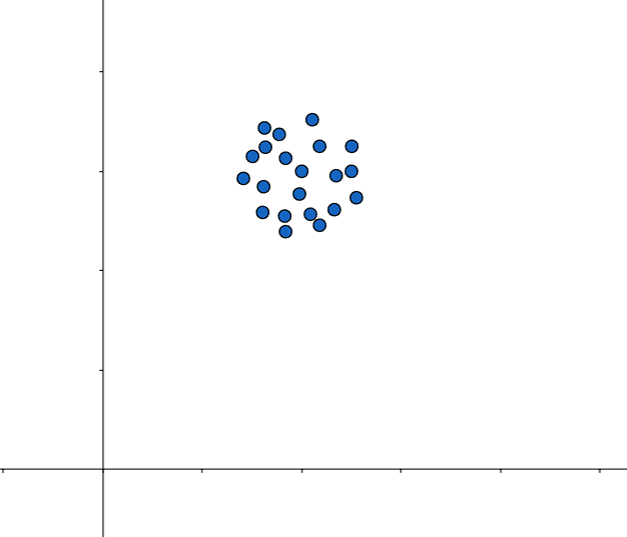
\includegraphics[height=5cm]{mathstat/images/mathstat_2025_04_01_1}

        Здесь, возможно, нет зависимости

        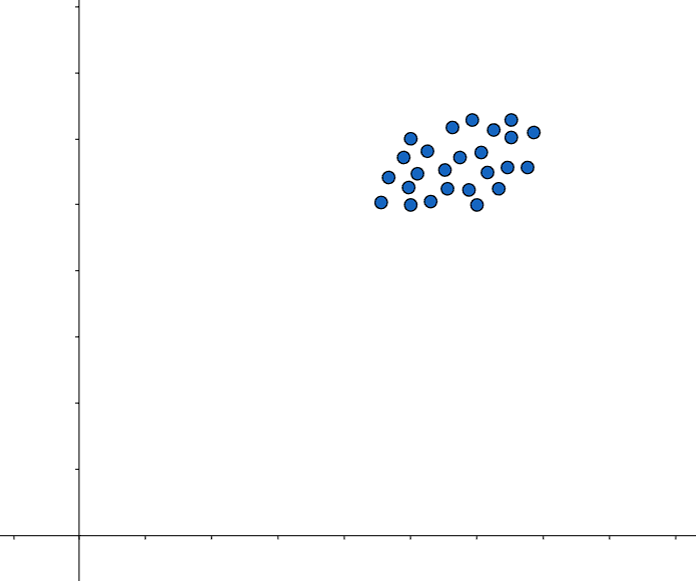
\includegraphics[height=5cm]{mathstat/images/mathstat_2025_04_01_2}

        Здесь можно предположить прямую корреляцию
    \end{center}
\end{multicols}

\subsection{Корреляционная таблица}

Пусть даны данные $X$ и $Y$ при $n$ экспериментов. Эти данные удобно представить в виде коррелеционной таблицы:
по вертикали отмечают различные значения $x$, а по горизонтали - $y$, в клетках таблицы отмечаются частота появления $n_{xy}$

\Ex $n = 50$

\smallvspace

\begin{tabular}{c|c|c|c|c|c|c}
    X\backslash Y & 10 & 20 & 30 & 40 & $n_x$ & $\overline y_x$ \\
    \hline
    2 & 7 & 3 & 0 & 0 & 10 & 13 \\
    \hline
    4 & 3 & 10 & 10 & 2 & 25 & 4.4 \\
    \hline
    6 & 0 & 2 & 10 & 3 & 15 & 30.67 \\
    \hline
    $n_y$ & 10 & 15 & 20 & 5 & $\Sigma$ 50 & \\
\end{tabular}

\smallvspace

По диагонали таблицы можно предположить, что корреляция есть

Имеет смысл вычислить условное среднее по формуле $\overline y (x) = \frac{1}{n_x} \sum n_{xy} y_i$. Так как в нашем примере
условные средние растут с ростом $x$, то имеет место прямая корреляция

\Nota Если данных много или $X$ и $Y$ -- непрерывные случайные величины, то лучше составить интервальную корреляционную таблицу:
разбить случайные величины на интервалы, по вертикали отметить интервалы $[a_{i - 1}, a_i)$ случайной величины $X$, 
по горизонтали -- $[b_{j - 1}, b_j)$ случайной величины $Y$, в клетках 
отметить частоты $n_{ij} : [a_{i - 1}, a_i) \times [b_{j - 1}, b_j)$. В дальнейшем интервалы можно заменить их серединами

\subsection{Критерий \enquote{хи-квадрат} для проверки независимости}

Пусть выборка $(X_1, Y_1), (X_2, Y_2), \dots, (X_n, Y_n)$ представлена в виде интервальной корреляционной таблицы. Случайная величина $X$ 
разбита на $k$ интервалов, а $Y$ -- на $m$ интервалов

Обозначим $v_{i\cdot}$ -- частота $i$-ого интервала $[a_{i - 1}, a_i)$ случайной величины $X$, 
$v_{\cdot j}$ -- частота $j$-ого интервала $[b_{j - 1}, b_j)$ случайной величины $Y$, $v_{ij}$ -- число точек в $[a_{i - 1}, a_i) \times [b_{j - 1}, b_j)$


\begin{tabular}{c|c|c|c|c|c}
    X\backslash Y & $[b_0, b_1)$ & $[b_1, b_2)$ & \dots & $[b_{m - 1}, b_m)$ & $v_{i\cdot}$ \\
    \hline
    $[a_0, a_1)$ & $v_{11}$ & $v_{12}$ & \dots & $v_{1m}$ & $v_{1\cdot}$ \\
    \hline
    \multicolumn{6}{c}{\dots} \\
    \hline
    $[a_{k - 1}, a_k)$ & $v_{k1}$ & $v_{k2}$ & \dots & $v_{km}$ & $v_{k\cdot}$ \\
    \hline
    $v_{\cdot j}$ & 10 & 15 & 20 & 5 & $\Sigma n$ \\
\end{tabular}

Проверяется основная гипотеза $H_0 : X \text{ и } Y$ независимы против $H_1 = \overline{H_0} : X \text{ и } Y$ зависимы

Если $H_0$ верна, то $p_{ij} = P(X \in [a_{i - 1}, a_i), Y \in [b_{j - 1}, b_j)) = P(X \in [a_{i - 1}, a_i)) \cdot P(Y \in [b_{j - 1}, b_j))$

Тогда по закону больших чисел $\frac{v_{i\cdot}}{n} \ConvergesInProbability p_{i\cdot}, \frac{v_{\cdot j}}{n} \ConvergesInProbability p_{\cdot j}$

Поэтому основанием для отклонения основной гипотезы будет заметная разница между величинами $\frac{v_{i\cdot}}{n}\frac{v_{\cdot j}}{n}$ и 
$\frac{v_{ij}}{n}$ или $v_{ij}$ и $\frac{1}{n} v_{i\cdot} v_{\cdot j}$

В качестве статистики берется $K = n \sum_{i, j} \frac{\left(v_{ij} - \frac{1}{n} v_{i\cdot} v_{\cdot j}\right)^2}{v_{i\cdot} v_{\cdot j}}$

\begin{MyTheorem}
    \Ths Если $H_0$ верна, то $K \rightrightarrows H_{(k - 1)(m - 1)}$
\end{MyTheorem}

Пусть $t_\alpha$ -- квантиль $H_{(k - 1)(m - 1)}$ уровня $\alpha$, тогда 

\begin{cases}
    H_0 : X \text{ и } Y \text{ независимы, если } K < t_\alpha \\
    H_0 : X \text{ и } Y \text{ зависимы, если } K \geq t_\alpha \\
\end{cases}

\Nota Для работы критерия необходимо, что бы частота в каждой клетке была больше 5, а объем выборки был достаточно большой

\subsection{Однофакторный дисперсионный анализ}

Предположим, что на случайную величину $X$ (результат) может влиять фактор $Z$ (необязательно, что $Z$ -- случайная величина, эксперимент может быть управляемым)

Пусть при различных \enquote{$k$ уровней} фактора $Z$ получено $k$ независимых выборок случайной величины $X$: 
$X^{(1)} = (X_1^{(1)}, \dots, X^{(1)}_{n_1}), \dots, X^{(k)} = (X_1^{(k)}, \dots, X^{(k)}_{n_k})$

Всего было получено $n = \sum_{i = 1}^k n_i$ значений

\Nota В общем говоря, распределение этих выборок отличается, поэтому эти выборки разных случайных величин

\subsubsection{Общая, внутригрупповая и межгрупповая дисперсии}

Для каждой выборки вычислим выборочное среднее и дисперсию: $\overline{x}^{(j)} = \frac{1}{n_j} \sum_{i = 1}^{n_j} X_i^{(j)}$, 
$D^{(j)} = \frac{1}{n_j} \sum_{i = 1}^{n_j} (X_i^{(j)} - \overline{x}^{(j)})^2$

Объединим все выборки в общую и также вычислим выборочнее среднее и дисперсию: 

$\overline{x} = \frac{1}{n} \sum_{i, j} x^{(j)}_i = \frac{1}{n} \sum_{j = 1}^k n_j \cdot \overline{x}^{(j)}$ - общее среднее

$D_\text{О} = \frac{1}{n} \sum_{i, j} (X^{(j)}_i - \overline{x})^2$ - общая дисперсия

\Def Внутригрупповой (или остаточной) дисперсией называется среднее групповых дисперсий: $D_{\text{В}} = \frac{1}{n} \sum_{j = 1}^k n_j D^{(j)}$

\Def Межгрупповой (или факторной) дисперсией называется величина $D_{\text{М}} = \frac{1}{n} \sum_{j = 1}^k n_j (\overline{x} - \overline{x}^{(j)})^2$

\begin{MyTheorem}
    \ThNs{О разложении дисперсии} Общая дисперсия равна сумме внутригрупповой и межгрупповой дисперсией: $D_\text{О} = D_\text{В} + D_\text{М}$
\end{MyTheorem}

Смысл: внутригрупповая дисперсия показывает средний (случайный) разброс внутри выборок, межгрупповая - насколько отличаются среднее при различных 
уровнях фактора, то есть именно эта величина отражает влияния фактора

Вывод по наличии корреляции можно сделать, если доля $D_\text{М}$ достаточно велика

\subsubsection{Проверка гипотезы о влиянии фактора}

Предполагаем, что $X$ имеет нормальное распределение и фактор $Z$ может влиять только на ее математическое ожидание, 
но на дисперсию и тип распределения, поэтому можно считать, что данные независимых $k$ выборок при различных уровнях фактора $Z$
также имеют нормальное распределение с одинаковой дисперсией: $X^{(j)} \in N(a_j, \sigma^2)$

Проверяется основная гипотеза $H_0 : a_1 = a_2 = \dots = a_k$ (фактор не оказывает влияния) против $H_1 = \overline{H_0} : $ есть влияние

По пункту 3 основной теоремы $\sum_{i = 1}^n \left(\frac{x_i - \overline{x}}{\sigma}\right)^2 = \frac{n D^*}{\sigma^2} \in H_{n - 1}$

Из этого $\frac{n_j D^{(j)}}{\sigma^2} \in H_{n_j - 1} \quad \forall \ 1 \leq j \leq k$

Так как распределение \enquote{хи-квадрат} устойчиво относительно суммирования, то $\sum_{j = 1}^k \frac{n_j D^{(j)}}{\sigma^2} \in H_{n - k}$, так как
$(n_1 - 1) + \dots + (n_k - 1) = n - k$

Пусть основная гипотеза верна, тогда все данные можно считать выборкой одной случайной величины и по пункту 3 $\frac{n D_{\text{О}}}{\sigma^2} \in H_{n - 1}$

Согласно теореме о разложении дисперсии $D_\text{О} = D_\text{В} + D_\text{М}$, тогда $\frac{n D_{\text{О}}}{\sigma^2} = \frac{n D_{\text{В}}}{\sigma^2} + \frac{n D_{\text{М}}}{\sigma^2}$

Так как $\frac{n D_{\text{О}}}{\sigma^2} \in H_{n - 1}, \frac{n D_{\text{В}}}{\sigma^2} \in H_{n - k}$, то $\frac{n D_{\text{М}}}{\sigma^2} \in H_{k - 1}$

Тогда при верной основной гипотезе получим, что $\frac{n D_{\text{М}}}{\sigma^2} \frac{\sigma^2 (n - k)}{n D_\text{В}} = \frac{n - k}{n - 1} \frac{D_\text{М}}{D_\text{В}} \in F(k - 1, n - k)$ --
распределение Фишера-Снедекера со степенями $k - 1$ и $n - k$

В качестве статистики берется $K = \frac{n - k}{n - 1} \frac{D_\text{М}}{D_\text{В}}$, в качестве критической точки $t_\alpha$ -- квантиль $F(k - 1, n - k)$ уровня $\alpha$

\begin{cases}
    H_0 : a_1 = a_2 = \dots = a_k \text{ (фактор оказывает влияние), если } K < t_\alpha \\
    H_0 : \text{фактор влияния не оказывает, если } K \geq t_\alpha \\
\end{cases}

% end mathstat_2025_04_01.tex



\end{document}

